% **************************************************
% Document Class Definition
% **************************************************
\documentclass[%
    paper=A4,               % paper size --> A4 is default in Germany
    twoside=true,           % onesite or twoside printing
    openright,              % doublepage cleaning ends up right side
    parskip=full,           % spacing value / method for paragraphs
    chapterprefix=true,     % prefix for chapter marks
    11pt,                   % font size
    headings=normal,        % size of headings
    bibliography=totoc,     % include bib in toc
    listof=totoc,           % include listof entries in toc
    titlepage=on,           % own page for each title page
    captions=tableabove,    % display table captions above the float env
    draft=false,            % value for draft version
]{scrreprt}%


% **************************************************
% Setup YOUR thesis document in this file !
% **************************************************
% !TEX root = my-thesis.tex


% **************************************************
% Files' Character Encoding
% **************************************************
\PassOptionsToPackage{utf8}{inputenc}
\usepackage{inputenc}


% **************************************************
% Information and Commands for Reuse
% **************************************************
\newcommand{\thesisTitle}{Costruzione di una base di conoscenza Linked Data con tecniche di Machine Learning}
\newcommand{\thesisName}{Lorenzo Franco Ranucci}
\newcommand{\thesisSubject}{Tesi di laurea}
\newcommand{\thesisCourse}{Corso di Laurea Magistrale in Informatica}
\newcommand{\thesisDate}{19 Aprile 2018}
\newcommand{\thesisVersion}{1}

\newcommand{\thesisFirstReviewer}{Prof.ssa Valentina Poggioni}
\newcommand{\thesisFirstReviewerUniversity}{\protect{Università degli Studi di Perugia}}
\newcommand{\thesisFirstReviewerDepartment}{Dipartimento di Matematica e Informatica}

\newcommand{\thesisSecondReviewer}{}
\newcommand{\thesisSecondReviewerUniversity}{\protect{Università degli Studi di Perugia}}
\newcommand{\thesisSecondReviewerDepartment}{Dipartimento di Matematica e Informatica}

\newcommand{\thesisFirstSupervisor}{}
\newcommand{\thesisSecondSupervisor}{}

\newcommand{\thesisUniversity}{\protect{Università degli Studi di Perugia}}
\newcommand{\thesisUniversityDepartment}{Dipartimento di Matematica e Informatica}
\newcommand{\thesisUniversityInstitute}{}
\newcommand{\thesisUniversityGroup}{}
\newcommand{\thesisUniversityCity}{Perugia PG}
\newcommand{\thesisUniversityStreetAddress}{Via Luigi Vanvitelli, 1}
\newcommand{\thesisUniversityPostalCode}{06123}


% **************************************************
% Debug LaTeX Information
% **************************************************
%\listfiles


% **************************************************
% Load and Configure Packages
% **************************************************
\usepackage[italian]{babel} % babel system, adjust the language of the content
\PassOptionsToPackage{% setup clean thesis style
    figuresep=colon,%
    sansserif=false,%
    hangfigurecaption=false,%
    hangsection=true,%
    hangsubsection=true,%
    colorize=full,%
    colortheme=bluemagenta,%
    bibsys=biber,%
    bibfile=bib-refs,%
    bibstyle=alphabetic,%
    wrapfooter=false,%
}{cleanthesis}
\usepackage{cleanthesis}

\hypersetup{% setup the hyperref-package options
    pdftitle={\thesisTitle},    %   - title (PDF meta)
    pdfsubject={\thesisSubject},%   - subject (PDF meta)
    pdfauthor={\thesisName},    %   - author (PDF meta)
    plainpages=false,           %   -
    colorlinks=false,           %   - colorize links?
    pdfborder={0 0 0},          %   -
    breaklinks=true,            %   - allow line break inside links
    bookmarksnumbered=true,     %
    bookmarksopen=true          %
}



% **************************************************
% Document CONTENT
% **************************************************
\begin{document}

% --------------------------
% rename document parts
% --------------------------
%\renewcaptionname{ngerman}{\figurename}{Abb.}
%\renewcaptionname{ngerman}{\tablename}{Tab.}
%\renewcaptionname{italian}{\figurename}{Fig.}
%\renewcaptionname{italian}{\tablename}{Tab.}

% --------------------------
% Front matter
% --------------------------
\pagenumbering{roman}			% roman page numbing (invisible for empty page style)
\pagestyle{empty}				% no header or footers

\begin{titlepage}
	\pdfbookmark[0]{Titlepage}{Titlepage}
	\tgherosfont
	\centering

	{\Large \thesisUniversity} \\[4mm]
	
\includegraphics[width=6cm]{gfx/logo.pdf} \\[2mm]
	\textsf{\thesisUniversityDepartment} \\
	\textsf{\thesisUniversityInstitute} \\
	\textsf{\thesisUniversityGroup} \\

	\vfill
    {\LARGE \thesisCourse \\[10mm]}
	{\large \thesisSubject} \\[5mm]
	{\LARGE \color{ctcolortitle}\textbf{\thesisTitle} \\[10mm]}
	{\Large \thesisName} \\

	\vfill
	\begin{minipage}[t]{.27\textwidth}
		\raggedleft
		\textit{Relatrice}
	\end{minipage}
	\hspace*{15pt}
	\begin{minipage}[t]{.65\textwidth}
		{\Large \thesisFirstReviewer} \\
	  	{\small \thesisFirstReviewerDepartment} \\[-1mm]
		{\small \thesisFirstReviewerUniversity}
	\end{minipage} \\[10mm]

	\thesisDate \\

\end{titlepage}


% ------------------------------------  --> lower title back for single page layout
\hfill
\vfill
{
	\small
	\textbf{\thesisName} \\
	\textit{\thesisTitle} \\
	\thesisSubject, \thesisDate \\
	Relatrice: \thesisFirstReviewer\\[1.5em]
	\textbf{\thesisUniversity} \\
	\thesisUniversityDepartment \\
	\thesisUniversityStreetAddress \\
	\thesisUniversityPostalCode\ \thesisUniversityCity
}


% !TEX root = ../my-thesis.tex
%
% ------------------------------------  --> cover title page
\begin{titlepage}
	\pdfbookmark[0]{Cover}{Cover}
	\flushright
	\hfill
	\vfill
	{\LARGE\thesisTitle \par}
	\rule[5pt]{\textwidth}{.4pt} \par
	{\Large\thesisName}
	\vfill
	\textit{\large\thesisDate} \\
	Versione: \thesisVersion
\end{titlepage}


% ------------------------------------  --> main title page
		% INCLUDE: all titlepages
\cleardoublepage

\pagestyle{plain}				% display just page numbers
% !TEX root = ../my-thesis.tex
%
\pdfbookmark[0]{Abstract}{Abstract}
\chapter*{Abstract}
\label{Abstract}
\vspace*{-10mm}

Questa ricerca si basa sull'intuizione che i risultati raggiunti nell'ambito della \textit{Knowledge Base Population} mediante \textit{Distant Supervision}, gli sviluppi introdotti dalla nuova tecnica di \textit{Data Programming} e l'efficienza dimostrata dalle \textit{Bidirectional Long Short Term Memory Network} (\textit{Bi-LSTM}) con input sequenziali come il testo libero, possano essere combinati per ottenere risultati allo stato dell'arte nella costruzione di basi di conoscenza \textit{Linked Data}. 

Il sistema software sviluppato fornisce una dimostrazione empirica di come una base di conoscenza \textit{Linked Data} come \textit{DBpedia} possa essere popolata con nuove triple, composte da predicati già definiti in un'ontologia \textit{OWL} (\textit{DBpedia Ontology}), analizzando testi enciclopedici scritti in linguaggio naturale (\textit{Wikipedia}). L'estrazione di tali informazioni avviene utilizzando tecniche di \textit{Natural Language Processing} (\textit{NLP}) e una rete neurale di tipo Bi-LSTM. In mancanza di dati naturalmente etichettati, si genera l'insieme di allenamento per il classificatore in maniera automatizzata secondo il paradigma di \textit{Data Programming} implementato nel framework \textit{Snorkel}.

Lo scopo del lavoro è quello di valutare il progetto sviluppato analizzando l'efficacia delle tecniche appena citate e confrontare i risultati con quelli riportati per i lavori allo stato dell'arte nella letteratura di competenza per la costruzione di basi di conoscenza.

 








		% INCLUDE: the abstracts (english and german)
\cleardoublepage
%
%% !TEX root = ../my-thesis.tex
%
\pdfbookmark[0]{Acknowledgement}{Acknowledgement}
\chapter*{Acknowledgement}
\label{sec:acknowledgement}
\vspace*{-10mm}

 % INCLUDE: acknowledgement
%\cleardoublepage
%
\setcounter{tocdepth}{2}		% define depth of toc
\tableofcontents				% display table of contents
\cleardoublepage

% --------------------------
% Body matter
% --------------------------
\pagenumbering{arabic}			% arabic page numbering
\setcounter{page}{1}			% set page counter
\pagestyle{maincontentstyle} 	% fancy header and footer


% !TEX root = ../my-thesis.tex
%
\chapter{Introduzione}
\label{sec:intro}
\cleanchapterquote{The Semantic Web is not a separate Web but an extension of the current one, in which information is given well-defined meaning, better enabling
computers and people to work in cooperation.}{Tim Berners-Lee}{}

Il Web, nei suoi quasi 30 anni di vita, si è evoluto da semplice archivio di documenti ipertestuali a base di conoscenza eterogenea. Questo cambiamento è stato graduale e non ha stravolto la struttura originaria del Web. Open Data e Semantic Web sono stati i due movimenti che hanno consentito congiuntamente la crescita di un Internet in cui uomini e macchine possono collaborare in maniera più efficace. Il contenuto Web è stato strutturato, arricchito da metadati, identificato univocamente, e collegato formando quelli che oggi vengono chiamati Linked Data.

Quello della generazione di Linked Data è un processo ancora in corso e che sta coinvolgendo sempre più organizzazioni, principalmente di tipo governativo, alimentando il concetto di Open Government. Sono stati  quindi delineati degli standard di creazione e distribuzione di Linked Data. 

Rendendo disponibili al pubblico dati che prima erano centralizzati e privati e donandogli una struttura interrogabile sia dall'intelligenza umana che da quella artificiale, cominciano a svilupparsi nuovi servizi in ambito culturale, scientifico, economico e governativo, permettendo partecipazione, trasparenza e condivisione.

In questo capitolo viene descritto come e perché il Web è evoluto in questa direzione, quali sono stati gli interessi e i precursori di questo cambiamento, come e da chi vengono prodotti oggi i Linked Open Data e quali sono i risultati e le sfide attuali.



\section{Storia del (Semantic) Web}
\label{sec:intro:web_history}

 
Il 6 Agosto 1991, presso il CERN, Tim Berners-Lee pubblica il primo sito web e mette a disposizione delle persone un innovativo e semplice mezzo di condivisione delle informazioni. 

Inizialmente il Web è stato usato in maniera molto semplice come grande archivio globale di documenti ipertestuali.
Il sistema di navigazione del web non forniva molte alternative: partendo da una risorsa documentale nota la si esplorava, tramite link, in cerca di nuove informazioni. 

In seguito l'indicizzazione degli indirizzi e la creazione dei motori di ricerca hanno introdotto la possibilità di interrogare la rete Internet e di cercare le informazioni in base a delle parole chiave. Tuttavia, pur avendo di molto ampliato le possibilità e il numero di utenti che ogni giorno utilizzano un browser, il tipo di interazione tra umano e macchina è rimasto ben diverso da quello tra persone.

Con l'avvento di database e linguaggi di programmazione Web, le informazioni digitali hanno cominciato a proliferare sia in ambito commerciale che di ricerca scientifica e ad adattarsi dinamicamente ad esigenze e comportamenti  dell'utente. 

Prima di proseguire è necessario marcare una linea di separazione tra i concetti di \textit{contenuto} o \textit{documento} e quello di \textit{dato}; adottando un’immagine proposta da Tim Berners-Lee, possiamo affermare che il contenuto è qualcosa che possiamo semplicemente leggere, mentre un dato può essere processato in differenti modi per creare nuova informazione.

I contenuti, pur provenendo molto spesso da basi strutturate di dati, hanno mantenuto per molto tempo l'esclusiva finalità di essere consultati dai soli utenti, rimanendo non processabili per le macchine. I dati invece hanno continuato ad avere le limitazioni di essere:
\begin{enumerate}
\item interrogabili dagli utenti finali esclusivamente tramite query predefinite dai progettisti e fornite sotto forma di interfacce web (form di ricerca),
\item centralizzati,
\item vincolati da licenze e diritti di autore,
\item scollegati da altri dati di altre fonti.
\end{enumerate}
Per combattere queste limitazioni, l'idea di accesso e riutilizzo libero e aperto che per tempo era stata associata al software (Open Source) è stata estesa al concetto di dato in generale, portando alla nascita del movimento Open Data.
Spesso i dati sono controllati da organizzazioni, sia pubbliche che private, che non ne consentono la consultazione e il riutilizzo. I sostenitori dell'idea di Open Data promuovono la cessazione di ogni limitazione di accesso a qualsiasi forma di dato, supportando una totale apertura. In particolare una delle organizzazioni internazionali di riferimento per il movimento, la \textit{Open Knowledge Foundation} \cite{okfn}, definisce gli Open Data e Open Content come: "dati e contenuti che possono essere liberamente usati, modificati e condivisi da chiunque e per qualsiasi motivo". Questo pensiero viene sempre di più assecondato e alimentato da enti governativi nazionali e internazionali, permettendo progressi in ambito culturale, scientifico, economico, ambientale e finanziario. 

Come Internet ha permesso la nascita del Web, gli Open Data hanno fornito l'infrastruttura perfetta per i Linked Data. Open Data ha reso i dati decentralizzati e accessibili a tutti, ma per arrivare ad un sistema di interrogazione potente e automatizzabile è necessario un ulteriore sviluppo. Proprio da colui che il Web l'ha inventato nasce la sua evoluzione: il \textit{Semantic Web} \cite{10.2307/26059207}\cite{semantic_web}\cite{Bizer2009LinkedD}\cite{BernersLee2006TabulatorEA}\cite{semantic_web_w3c}.
Il movimento per il Semantic Web è interessato a compiere questo processo di trasformazione del documento in dato, trasformando il Web da archivio documentale a database distribuito.
Per far funzionare il Semantic Web, i computer devono avere accesso a collezioni strutturate di informazioni e insiemi di regole di inferenza per condurre deduzioni automatiche. I ricercatori di Intelligenza Artificiale hanno studiato per anni questa tecnologia denominata \textit{rappresentazione della conoscenza}, anche prima della nascita del Web. L'ambizione è quella di stimolare le organizzazioni mondiali di ogni genere a contribuire alla costruzione di una base di conoscenza condivisa, sia per le persone che per i computer, al fine di favorire la qualità della loro cooperazione.
Il contenuto di un documento Web moderno, pur provenendo da fonti strutturate come database, perde il suo significato semantico e relazionale intrinseco nel momento in cui viene espresso sotto forma di documento HTML. Per valorizzare il dato è importante che esso:

\begin{itemize}
\item abbia una struttura standard,
\item venga corredato da metadati standard,
\item sia identificabile,
\item sia collegato ad altri dati.
\end{itemize}

Gli sforzi provenienti dai movimenti Open Data e Semantic Web si fondono così sotto il nome di Linked Open Data. Tim Berners-Lee formula una classificazione a "5 stelle" per gli Open Data, in cui il livello Linked è proprio quello più avanzato \cite{5_star_open_data}. I primi tre livelli definiscono gli Open Data come:
\begin{enumerate}
\item accessibili in rete,
\item comprensibili da un calcolatore,
\item in un formato non proprietario.
\end{enumerate}
Gli ultimi due livelli invece stabiliscono che per essere Linked, un dato deve essere inoltre nel formato standard prestabilito \textit{RDF} e collegato ad altre risorse. Un dato isolato possiede poco valore, ma se "linkato" ad altri dati assume nuovi significati deducibili dal grafo di dati a cui è connesso.

\begin{figure}[htb]
	\fbox{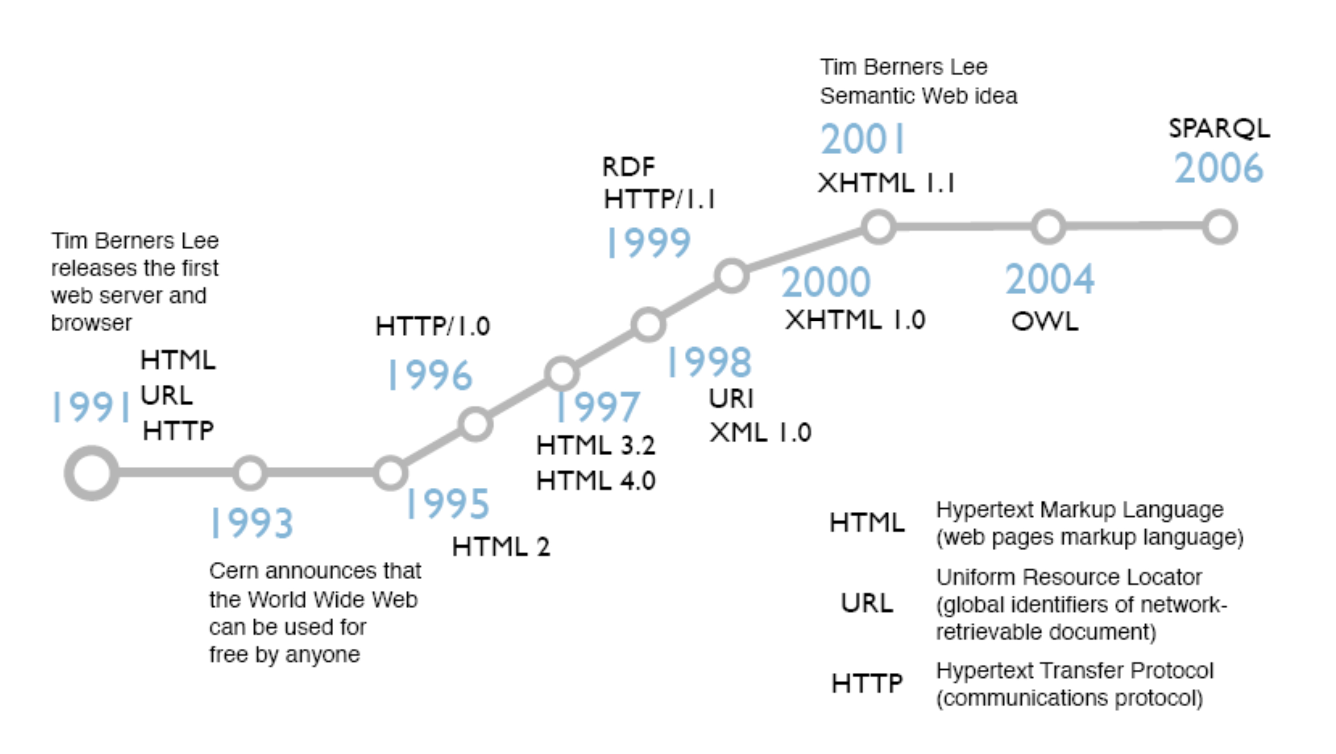
\includegraphics[width=\textwidth]{gfx/web_timeline.pdf}}
	\caption{Web timeline}
	\label{fig:introduction:web_timeline}
\end{figure}


Per capire le potenzialità del Web Semantico basta pensare a un episodio che è probabile vivere nell'interazione con un motore di ricerca: fare richieste basate sul significato invece che sulle parole chiave del tipo "Chi è l'inventore del Web?". Una simile interrogazione avrebbe prodotto in passato risultati tutt'altro che precisi, richiedendo la lettura all'interno dei documenti restituiti come risultato o la formulazione di una nuova ricerca. Il motivo era dovuto alla mancanza di struttura semantica nei documenti HTML indicizzati dai motori di ricerca.
Quello che invece otteniamo oggi è proprio la risposta "Tim Berners-Lee" (Fig. \ref{fig:introduction:ricerca_semantica}), come se il nostro interlocutore fosse una persona informata sulla storia del Web.

\begin{figure}[htb]
	\fbox{
\includegraphics[width=\textwidth]{gfx/ricerca_semantica.pdf}}
	\caption{Ricerca semantica}
	\label{fig:introduction:ricerca_semantica}
\end{figure}

Questo risultato che può sembrare irrilevante all'utente meno fantasioso, è in realtà di incredibile importanza ed è frutto di un meccanismo di inferenza che coinvolge Linked Data e Intelligenza Artificiale. Tale logica è estendibile, per esempio, a insiemi di dati di rilevanza nell'ambito della ricerca e provenienti da fonti diverse, trasformando dati che prima erano slegati e strutturati secondo la logica decisa dalla fonte (e quindi interrogabili solo avendone diritto d'accesso e conoscendo la struttura specifica), in dati collegati e interrogabili con un processo di inferenza semantica affine a quello della mente umana.

Il meccanismo di interrogazione si evolve da semplice ricerca di termini chiave a qualcosa di più elaborato. Il linguaggio naturale della query viene analizzato con tecniche di \textit{NLP (Natural Language Processing)}, scomponendone il testo, definito in ambito linguistico come proposizione, nella sua struttura fondamentale "soggetto-predicato-oggetto". Nel caso della domanda precedente, il soggetto è l'incognita che l'utente vuole conoscere, il predicato è "essere inventore" e l'oggetto è "il Web".
Immaginiamo ora una base di conoscenza in cui i dati siano strutturati considerando come modello proprio la proposizione. Per dare una risposta alla domanda, sarebbe sufficiente trovare tutte le triple "soggetto-predicato-oggetto" che abbiano predicato e oggetto come sopra e restituire come risultato ciascun soggetto. Ebbene questo formato è proprio lo standard del Semantic Web e dei Linked Data: RDF. 

\section{Struttura standard del Semantic Web}
\label{sec:intro:web_history}

Il modello \textbf{\textit{RDF}} (\textit{Resource Description Framework})\cite{rdf_overview}, rappresenta l'informazione in maniera simile a come viene espressa dalla logica umana, sotto forma di asserzioni (o proposizioni) composte da \textit{soggetto}, \textit{predicato} e \textit{oggetto}. Il modello RDF viene serializzato in diversi tipi di formato che non ne alterano la logica e sono intercambiabili. I formati più popolari per la serializzazione di modelli RDF sono: \textit{RDF/XML, Turtle, NTriples}.

Il lettore più scrupoloso avrà certamente obiettato, nella scorsa sezione, che il linguaggio naturale è per natura ambiguo e quindi inadatto ad un processo di inferenza. Per questo motivo, nella progettazione delle basi di conoscenza Linked Data, si è scelto di usare come classe di dato fondamentale quella che viene chiamata \textit{entità} o \textit{nodo}. Tali entità possono essere usate come soggetto e oggetto di una tripla. Per essere distinte in maniera non ambigua vengono etichettate con degli \textit{\textbf{URI} (Universal Resource Identifier)}. 
Queste entità rappresentano qualsiasi concetto del mondo reale. 
Dato che gli RDF usano URI per codificare le informazioni, ci si assicura che i concetti non siano solo parole in un documento, ma che siano unicamente identificati, referenziabili da altre risorse e disponibili nel Web (nel caso in cui un URI sia specializzato in un URL HTTP). 


\iffalse
\begin{figure}[htb]
	
   \fbox{ includegraphics[width=\textwidth]{gfx/LOV.pdf} }
	\caption{Grafo Linked Open Vocabularies (Ontologie)}
    {Mostra tutte le ontologie OWL esistenti}
    {(\textit{Linking Open Data cloud diagram 2017, by Andrejs Abele, John P. McCrae, Paul Buitelaar, Anja Jentzsch and Richard Cyganiak. http://lod-cloud.net/})}
	\label{fig:introduction:lov}
\end{figure}
\fi

Come già detto, i dati presenti in un database sono strutturati, ma fare Linked Open Data non significa solamente diffondere tali dati pubblicamente, ma farlo utilizzando una struttura e dei significati (metadati) condivisi da tutti. Se il problema di avere una struttura standard viene risolto dall'uso dell'RDF, quello di fornire tipi di metadati standard, dare significato e definire regole di inferenza viene assolto dalle \textit{ontologie} (o \textit{vocabolari}) \textit{OWL} \cite{w3c_owl}. 

Invece di utilizzare nomi di \textit{proprietà} (\textit{predicati} o \textit{relazioni}) diversi per lo stesso concetto, la comunità scientifica lavora alla definizione di insiemi di proprietà per tipi di concetti diversi. E' così che anche l'ambiguità di descrivere la stessa proprietà con parole diverse viene superata utilizzando predicati creati appositamente da organizzazioni autorevoli, identificati da URI e non ripetuti. Un'ontologia è, in altre parole, una tassonomia che esprime il significato semantico e le relazioni di una categoria omogenea di dati.

Ricapitolando, i Linked Data sono composti da due insiemi di dati etichettati da URI: le \textit{entità} (o \textit{nodi}) e le \textit{proprietà} (o \textit{predicati}). Coppie di entità possono essere relazionate tra loro dalle proprietà. 

Esistono anche delle entità speciali che non sono identificate da 
URI: \nolinebreak
\begin{itemize}
\item \textit{Literal}: dati primitivi testuali come numeri, date o nomi propri.
\item \textit{Blank Nodes}: nodi anonimi usati solitamente come nodi strutturali ausiliari di nodi complessi.
\end{itemize}

Formalmente \cite{RDF_DEFINITION} un RDF è definito come una raccolta di triple. Un insieme di tali triple è definito \textit{Grafo RDF}. 
Una \textit{tripla RDF} contiene tre componenti ordinate:
\begin{enumerate}
\item il \textit{soggetto}, che è un \textit{URI RDF} o un \textit{Blank node};
\item il \textit{predicato} (o \textit{proprietà}) che è un \textit{URI RDF} (definito in un'ontologia);
\item l'\textit{oggetto} che è un \textit{URI RDF} o un \textit{Blank node} o un \textit{Literal}.
\end{enumerate}
Per convenzione ci si riferisce ad una tripla RDF con la notazione \textit{(s, p, o)}.
\begin{figure}[htb]
	\fbox{
\includegraphics[width=\textwidth]{gfx/rdf_triple_example.pdf}}  
	\caption{Tripla RDF}
	\label{fig:introduction:rdf_triple}
\end{figure}



A livello intuitivo una tripla può essere illustrato da un grafo orientato in cui ogni tripla soggetto-predicato-oggetto è rappresentata come nodo-arco-nodo  (Fig. \ref{fig:introduction:rdf_triple}). L'intero database globale di Linked Data può essere visto come una grande tabella di tre colonne oppure come un grande grafo (Fig. \ref{fig:introduction:lod}).
Si noti che i literal possono comparire solamente come oggetto delle triple e quindi come nodi foglia del grafo.

\begin{figure}[htb]
	\fbox{\includegraphics[width=\textwidth]{gfx/lod.pdf} }
	\caption{Grafo Linked Opend Data}
	\label{fig:introduction:lod}
\end{figure}


Come spiegato in precedenza, il fine di quanto descritto finora è quello di sviluppare un sistema che consenta una migliore interoperabilità tra programmi e persone e tra programmi ed altri programmi. Costruire quindi un sistema che cataloghi con una struttura condivisa (RDF) tutta la conoscenza umana, ne delinei la semantica e le regole di inferenza per le intelligenze artificiali (OWL) e la renda interrogabile (SPARQL). 


Così come RDF è il formato strutturale standard per il Semantic Web, \textbf{\textit{SPARQL}} (\textit{Simple Protocol And RDF Query Language}) \cite{sparql_overview} è un insieme di specifiche standard che definisce:
\begin{itemize}
\item il linguaggio di interrogazione e aggiornamento \textit{SPARQL Query/Update Language} ;
\item la struttura \textit{graph store}  in cui i dati RDF sono organizzati in sottografi identificati da URI;
\item il protocollo \textit{SPARQL Protocol} che definisce il motore di interrogazione e le comunicazioni \textit{SPARQL Graph Store HTTP Protocol}.
\end{itemize}
Questi servizi vengono resi accessibili al pubblico sotto forma di interfaccia Web e servizio REST in quello che viene definito \textit{SPARQL Endpoint}.
Il linguaggio SPARQL consente di effettuare interrogazioni che vanno dalla semplice corrispondenza di pattern su grafi, a query complesse usando operatori comuni ai linguaggi relazionali. 
Fare una interrogazione in SPARQL vuol dire navigare il grafo lungo gli archi ed i nodi fino a soddisfare tutti i vincoli dell’inferenza e restituire il grafo attraversato. Le richieste vengono serializzate mediante il formato \textit{Turtle}, mentre il risultato della richiesta può essere una tabella in diversi formati (JSON, HTML, XML, CVS) o un sotto-grafo.

L'utilizzo di proprietà, definite nelle ontologie, nella costruzione dei Linked Data, rendono l'interrogazione SPARQL in grado di effettuare l'inferenza di proprietà non esplicitamente espresse dalle entità (Esempio in figura \ref{fig:introduction:rdf_graph}).

La specifica \textit{SPARQL Federated Query} consente l'interrogazione dell'intero grafo globale avendo come unico punto di accesso un singolo SPARQL Endpoint.


\begin{figure}[htb]
\begin{tikzpicture}[node distance=2.75cm,>=stealth']
\node[vertex style=Turquoise] (Rk) {dbr:Zinédine Zidane};

\node[vertex style=BurntOrange, above of=Rk,xshift=15.5em, yshift=3.5em] (BD) {dbr:Real\_Madrid\_C.F.}
 edge [<-,cyan!60!blue] node[text style]{dbo:team} (Rk);

\node[vertex style=BurntOrange, right=2.5cm of Rk,yshift=4ex] (AP) {dbr:Juventus\_F.C.}
 edge [<-,cyan!60!blue] node[text style]{dbo:team} (Rk); 

\node[vertex style=red, below right of=Rk,xshift=9em, yshift=-6em] (JA) {dbr:Midfielder}
 edge [<-,cyan!60!blue] node[text style]{dbo:position} (Rk); 

 \node[vertex style=BurntOrange, right=2.0cm of Rk,yshift=-4em] (RN) {dbr:FC\_Girondins\_de\_Bordeaux}
 edge [<-,cyan!60!blue] node[text style]{dbo:team} (Rk); 

\node[vertex style=MidnightBlue, above left of=Rk,xshift=2em, yshift=4em] (Dr) {"Zinedine Zidane"@en}
 edge [<-,cyan!60!blue] node[text style]{rdfs:label} (Rk); 

\node[vertex style=Maroon, below of=Rk,xshift=-2em] (Skf) {dbo:Athlete}
 edge [<-,cyan!60!blue] node[text style]{rdf:type} (Rk);

\node[vertex style=Maroon, below right of=Skf, yshift=-4em] (Cf) {dbo:Person}
 edge [<-,cyan!60!blue] node[text style]{rdfs:subClassOf} (Skf);

\begin{pgfonlayer}{background}
\draw[Maroon,fill=Maroon,dashed,fill opacity=0.1](Rk.north) 
to[closed,curve through={(Rk.north west).. (Rk.west) .. (Rk.south west) 
..($(Rk.south west)!0.5!(Skf.north)$) .. (Skf.north     west).. (Skf.west) 
.. (Skf.south west) .. ($(Skf.south)!0.75!(Cf.west)$) .. (Cf.west) 
.. (Cf.south west) .. (Cf.south) .. (Cf.south east) .. (Cf.east) 
.. ($(Cf.north east)!0.65!(Skf.south east)$) .. (Skf.east) 
.. (Skf.north east).. ($(Skf.north)!0.35!(Rk.south east)$) 
.. (Rk.south east) .. (Rk.east)..(Rk.north east)}](Rk.north);
\end{pgfonlayer}

\end{tikzpicture}
	\caption{Inferenza SPARQL}{L'area con sfondo marrone indica un passo di inferenza. Il tipo \textit{Person}, può essere dedotto dal tipo \textit{Athlete} direttamente collegato all'entità RDF presa in considerazione}
	\label{fig:introduction:rdf_graph}
\end{figure}

\section{Creazione e pubblicazione dei Linked Data}
\label{sec:intro:linked_data_production}

Sarebbe auspicabile che tutte le organizzazioni mondiali seguissero le indicazioni della comunità per il Semantic Web permettendo la costruzione di basi di conoscenza più complete e servizi, che le sfruttano, sempre più avanzati. A maggior ragione, il cittadino dovrebbe pretendere che questo avvenga per quelle organizzazioni che sono di origine pubblica. Questa legittima pretesa ha dato origine all'idea di \textit{Open government} che, in linea con il movimento open in generale, cerca di rendere il lavoro dei governi trasparente, responsabile, comprensivo e partecipativo per il cittadino. Come conseguenza a questa esigenza e opportunità, organizzazioni governative (come AGID in Italia) e non (Open Knowledge International) si sono attivate per il perseguimento delle politiche Open Data, elaborando linee guida e fornendo risorse di supporto.

Linee guida per la pubblicazione di Open Data a livello Linked sono state formulate da Tim Berners-Lee\cite{5_star_open_data} sotto forma di quattro semplici regole:
\begin{enumerate}
\item usare gli URI per identificare i dati;
\item usare URI HTTP (URL) in modo che le persone possano "visitare" questi dati usando un semplice browser;
\item le risorse identificate da URI devono fornire informazioni utili utilizzando gli standard RDF e SPARQL;
\item includere URI che collegano i dati tra loro, in modo da estendere il sistema sul quale fare inferenza \label{sec:intro:link_discovery}.
\end{enumerate}

Un'altra buona abitudine è quella di riutilizzare il più possibile gli URI già esistenti e fare collegamenti ad altre fonti. In questo modo il grafo globale Linked Data si mantiene più connesso e meno spazioso e di conseguenza più veloce ed interessante da interrogare.
Oltre alle linee guida per la strutturazione del dato, varie organizzazioni hanno formulato specifiche per l'intero processo produttivo di Linked Open Data.

%%Nuova sezione
Per esaminare il processo di produzione dei Linked Data ci si riferisce nel resto di questa sezione al caso reale di generazione dei Linked Open Data della Regione Umbria. Esso ci consente un'analisi senza perdita di generalità in quanto svolto in conformità alle linee guida delineate dall'AGID  e in ottemperanza alla direttiva Europea 2013/37/UE, detta PSI 2.0, che impone alle pubbliche amministrazioni azioni finalizzate al riutilizzo dei dati pubblici anche per fini commerciali. 

\subsection{Linked Open Data della Regione Umbria}
\label{sec:intro:linked_data_production:RU}

La Regione Umbria ha intrapreso fin dal 2014 il percorso di apertura dei dati regionali attraverso il programma \#opendata dell’Agenda Digitale Umbra. Grazie alla collaborazione con \textit{Umbriadigitale s.c.a r.l.} e con il \textit{Dipartimento di Informatica, Sistemistica e Comunicazione dell’Università Milano Bicocca} a poco tempo dall’avvio del percorso, si è giunti a creare l’ambiente tecnico e metodologico che ha permesso di pubblicare i primi Linked Open Data nel portale regionale. Questo meccanismo di produzione e pubblicazione dei Linked Data della Regione Umbria è attualmente assolto da un progetto gestito dall'Ing. Azzurra Pantella di Umbria Digitale, a cui l'autore di questa tesi ha l'opportunità di collaborare.

La Regione Umbria segue il modello ODMC (Open Data Management Cycle) \cite{ODMC} che delinea l'intera organizzazione per la gestione di Open Data. Si tratta di un processo ciclico composto da quattro punti:
\begin{enumerate}
\item identificazione dei dataset da pubblicare, richiedendo la partecipazione diretta del cittadino alla proposta di essi;
\item analisi della disponibilità, del valore e della qualità dei dati richiesti ed eventuale pubblicazione;
\item monitoraggio delle performance dei dataset;
\item mantenimento, aggiornamento ed eventuale dismissione  dei dati pubblicati.
\end{enumerate}


Il software open source CKAN \cite{CKAN} rappresenta un elemento di centrale importanza nell'implementazione di tale modello. CKAN permette di catalogare i dataset e descriverli attraverso una serie di metadati che da un lato aiutano gli utenti a navigare tra le informazioni e dall’altro favoriscono l’indicizzazione degli stessi dataset sui motori di ricerca. Sono molti, e in continuo aumento, gli enti pubblici che hanno adottato CKAN per esporre il proprio patrimonio informativo in formato Open Data, rendendolo uno standard \textit{de facto}\cite{ckan_agid}.
Il portale \textit{dati.umbria.it }\cite{datiumbria} è il punto di accesso per il cittadino ai Linked Open Data della Regione Umbria. E' un portale costruito su CKAN ed implementa, tra l'altro, il primo punto del modello ODMC sopra esposto fornendo un form per la proposta da parte del cittadino della messa a disposizione di nuovi dataset; quelli proposti e valutati positivamente, una volta estratti e strutturati, vengono pubblicati su questa piattaforma.

Una volta superato il processo di verifica della disponibilità e attestazione di utilità del dataset, si innesca il processo di analisi del dato. I dati sorgente possono essere generalmente immagazzinati in: database, file strutturati, file non strutturati (documenti di testo libero) o documenti cartacei. Ad oggi i soli dati che vengono trasformati in Linked Data sono quelli disponibili in formato strutturato (file o database). Per i dati non strutturati non esistono ancora soluzioni in grado di fornire un processo adeguatamente rapido, automatizzato, accurato e poco dispendioso di trasformazione. Quello di estrarre informazioni strutturate da documenti non strutturati è un problema attuale a cui si cerca di dare un contributo in questo lavoro.

I dati strutturati vengono sottoposti ad un processo di ETL (Extract Transform Load) usando il framework \textit{UnifiedViews} \cite{unifiedviews}. Le basi di dati vengono denormalizzate, se 
necessario, e viene fatta una selezione delle tabelle le cui tuple siano da pubblicare. Ciascuna tupla selezionata verrà poi trasformata, alla fine del processo, in nodo RDF.

Per ogni collezione di entità selezionate si sceglie innanzitutto l'ontologia adatta a descriverle. Si selezionano come prime proprietà i predicati \textit{<http://www.w3.org/1999/02/22-rdf-syntax-ns\#type>} che identificano le classi che l'oggetto istanzia. Per esempio, per una tabella di ricercatori scientifici si potrebbe scegliere di estrarre entità del tipo \textit{<http://xmlns.com/foaf/0.1/Person>}. Di conseguenza si controllano quali proprietà della classe definita nell'ontologia è possibile soddisfare con i dati del database. Se nella tabella considerata in precedenza è presente la colonna "nome" si potrà valorizzare l'oggetto per il predicato \textit{<http://xmlns.com/foaf/spec/\#term\_firstName>}. Si ipotizzi di avere una tabella che associa i propri ricercatori con quelli di altre organizzazioni in base alle pubblicazioni che essi hanno sostenuto insieme. Se tali ricercatori hanno già una risorsa RDF che li identifica in un dataset di una fonte esterna, è possibile usare link \textit{<http://purl.org/net/soron/workPartnerOf>} che hanno come oggetto gli URI dei ricercatori esterni. Questo processo si chiama \textit{Link Discovery} ed è di fondamentale importanza per rispettare la quarta regola proposta da Tim Berners-Lee e dare valore "deducibile" ai dati pubblicati.

Al termine di questa fase di trasformazione, i dataset generati possono essere caricati sia sul catalogo CKAN che sul graph store \textit{Virtuoso Universal Server} \cite{virtuoso}. Virtuoso è un database che offre, tra le molte funzionalità, la possibilità di memorizzare, organizzare e interrogare dati RDF. Implementa quindi un motore SPARQL, e permette di organizzare i vari dataset in (sotto-)grafi identificati da URI. Il punto di accesso al motore SPARQL è un servizio REST denominato SPARQL Endpoint. 
La procedura di estrazione, trasformazione e caricamento dei Linked Data è interamente assolta da UnifiedViews definendo delle \textit{pipeline}. L'integrabilità di UnifiedViews con CKAN fa in modo che il caricamento dei dataset prodotti avvenga come un passaggio della pipeline. Lo stesso vale per Virtuoso, supportato da UnifiedViews come client. 

L'aggiornamento dei dati è reso fattibile dalla possibilità di schedulare l'esecuzione delle pipeline in UnifiedViews.

La pubblicazione dei dataset viene conclusa con l'attribuzione di una licenza open.

\section{Interrogazione dei Linked Data}
\label{sec:intro:sparql}



In questa sezione viene mostrato un caso d'uso generico dello SPARQL Query Language. Come nella sezione precedente si farà riferimento ai dati della Regione Umbria.

Il protocollo SPARQL consiste di due operazioni: \textit{query} e \textit{update}. Queste operazioni devono essere invocate e servite via HTTP GET o HTTP POST. Il punto di accesso HTTP al servizio SPARQL si chiama \textit{SPARQL Endpoint} e viene messo a disposizione del pubblico dalle organizzazioni che conservano i propri dati in un graph store. Il graph store più popolare, di cui fa uso anche la Regione Umbria, è il già citato Virtuoso. Lo SPARQL Endpoint permette a qualsiasi utente di interfacciarsi con il graph store ed interrogarne i dati e viene pubblicato per convenzione sotto il percorso \textit{"/sparql"}, nel caso specifico \textit{https://dati.umbria.it/sparql}.

Lo SPARQL Endpoint è composto da:
\begin{enumerate}
\item un input testuale per la definizione del grafo da interrogare di default (\textit{default-graph-uri}),
\item un'area testuale per l'inserimento della query,
\item un menu per la selezione del formato del risultato.
\end{enumerate}
Il meccanismo principale per calcolare il risultato delle query SPARQL è chiamato \textit{subgraph matching}.
Fare un'interrogazione in SPARQL vuol dire navigare il grafo lungo gli archi ed i nodi fino a soddisfare tutti i vincoli dell’inferenza e restituire il grafo attraversato.
Secondo questo meccanismo l'utente decide innanzitutto quali sottografi interrogare, selezionando quindi un insieme di triple RDF. Il modello della query può contenere delle variabili usate come \textit{wild cards}. Nel linguaggio SPARQL le variabili sono identificate dal simbolo "?" usato come prefisso (es. ?subject).
Il sottografo risultante deve combaciare sia con un sottografo del sottografo di partenza che con il grafo modellato dalla query.
Grazie alla struttura RDF e alle regole OWL che forniscono una interpretazione semantica per i dati, è possibile inferire nuove triple RDF implicite a partire dalle asserzioni esplicitamente dichiarate.

Come già spiegato, in un graph store i dati RDF sono organizzati in sottografi identificati da URI.
La prima cosa da fare quando si decide di interrogare un graph store che non si conosce è scoprire quali sottografi contiene. Per farlo si esegue la query in \ref{lst:intro:sparql1}, senza specificare nessun grafo di default.\\ 



\lstset{ basicstyle=\LSTfont, columns=fullflexible, xleftmargin=5mm, framexleftmargin=5mm, numbers=left, stepnumber=1, breaklines=true, breakatwhitespace=false, numberstyle=\footnotesize, numbersep=5pt, tabsize=2, frame=lines, captionpos=b}
   
\begin{lstlisting}[frame=single, caption={Individuare i grafi salvati in un graph store.},label={lst:intro:sparql1},]  
SELECT DISTINCT ?graph
WHERE{
	GRAPH ?graph {?s ?p ?o}
}
\end{lstlisting}

\begin{table}[htbp]
\begin{center}
\begin{tabular}{|l|}
\hline \textbf{?graph} \\
\hline
http://dati.umbria.it/graph/consorzi\\
\hline
http://dati.umbria.it/graph/impianti\_sportivi\\
\hline
http://dati.umbria.it/graph/attrattori\\
\hline
...\\
\hline
%table & tabelle \\
\end{tabular}
\end{center}
\caption{Risultato \textit{Snippet \ref{lst:intro:sparql1}}}
\label{tab:intro:sparql1}
\end{table}

Si sceglie poi il grafo di interesse da interrogare e si usa come grafo di default. Si procede con l'esaminare i tipi di dato contenuti nel grafo selezionato (Snippet \ref{lst:intro:sparql2}).


\begin{lstlisting}[frame=single, caption={Individuare i tipi di dato del grafo scelto.},label={lst:intro:sparql2}]  
#default-graph-uri=http://dati.umbria.it/graph/attrattori

SELECT DISTINCT ?o
WHERE{
	?s <http://www.w3.org/1999/02/22-rdf-syntax-ns#type> ?o .
}
\end{lstlisting}

\begin{table}[htbp]
\begin{center}
\begin{tabular}{|l|}
\hline \textbf{?o} \\
\hline
http://linkedgeodata.org/ontology/Attraction\\
\hline
http://dati.umbria.it/tourism/ontology/descrizione\\
\hline
http://dati.umbria.it/tourism/ontology/tempo\_di\_viaggio\\
\hline
...\\
\hline
%table & tabelle \\
\end{tabular}
\end{center}
\caption{Risultato \textit{Snippet \ref{lst:intro:sparql2}}}
\label{tab:intro:sparql2}
\end{table}

Scegliendo un tipo di dato si possono ottenere tutti i nodi del grafo che istanziano tale classe (Snippet \ref{lst:intro:sparql3}).
\begin{lstlisting}[frame=single, caption={Individuare i nodi del tipo scelto.},label={lst:intro:sparql3}]  
#default-graph-uri=default-graph-uri=http://dati.umbria.it/graph/attrattori

SELECT DISTINCT ?s 
WHERE{
    ?s  <http://www.w3.org/1999/02/22-rdf-syntax-ns#type> <http://linkedgeodata.org/ontology/Attraction> .
}
\end{lstlisting}

\begin{table}[htbp]
\begin{center}
\begin{tabular}{|l|}
\hline \textbf{?s} \\
\hline
http://dati.umbria.it/risorsa/attrattori/101037\\
\hline
http://dati.umbria.it/risorsa/attrattori/101047\\
\hline
http://dati.umbria.it/risorsa/attrattori/101057\\
\hline
...\\
\hline
%table & tabelle \\
\end{tabular}
\end{center}
\caption{Risultato \textit{Snippet \ref{lst:intro:sparql3}}}
\label{tab:intro:sparql3}
\end{table}

Si possono poi ottenere tutte le proprietà di un nodo scelto (Snippet \ref{lst:intro:sparql4}).

\begin{lstlisting}[frame=single, caption={Ottenere i valori delle proprietà del nodo scelto},label={lst:intro:sparql4}]  
#default-graph-uri=default-graph-uri=http://dati.umbria.it/graph/attrattori

SELECT DISTINCT ?p ?o
WHERE{
    <http://dati.umbria.it/risorsa/attrattori/117043> ?p ?o.
}
\end{lstlisting}

\begin{table}[htbp]
\begin{center}
\begin{tabular}{|l|l|}
\hline \textbf{?p} & \textbf{?o} \\
\hline
.../rdf-schema\#label &	"Die Fontana Maggiore in Perugia"@de\\
\hline
.../rdf-schema\#label &	"Fontana Maggiore a Perugia"@it\\
\hline
.../rdf-schema\#label &	"The Fontana Maggiore in Perugia"@en\\
\hline
.../owl\#sameAs &	http://dbpedia.org/resource/Fontana\_Maggiore\\
\hline
...&...\\
\hline
%table & tabelle \\
\end{tabular}
\end{center}
\caption{Risultato \textit{Snippet \ref{lst:intro:sparql4}}}
\label{tab:intro:sparql4}
\end{table}

Si noti come nel risultato \ref{tab:intro:sparql4} compaia la proprietà \textit{sameAs}, che ha come oggetto una risorsa di un dataset di una fonte esterna che è DBpedia.
L'estensione \textit{SPARQL Federated Query} \cite{SPARQL_FEDERATED_QUERY}, consente all'autore della query di dirigere una parte di essa ad uno SPARQL Endpoint specifico e diverso da quello che si sta utilizzando. Tale estensione ricombina poi i vari sottorisultati in un solo grafo. Si possono così inferire nuove proprietà a partire dalla proprietà \textit{sameAs} ottenuta in precedenza (Snippet \ref{lst:intro:sparql5}).

\begin{lstlisting}[frame=single, caption={Query federata},label={lst:intro:sparql5}]  
#default-graph-uri=default-graph-uri=http://dati.umbria.it/graph/attrattori

SELECT DISTINCT ?pDBpedia ?oDBpedia
WHERE{   
    <http://dati.umbria.it/risorsa/attrattori/117043> <https://www.w3.org/2002/07/owl#sameAs> ?o.
    SERVICE <http://dbpedia.org/sparql> { 
		?o ?pDBpedia ?oDBpedia . 
    } 
}
\end{lstlisting}

\begin{table}[htbp]
\begin{center}
\begin{tabular}{|l|l|}
\hline \textbf{?pDBpedia} & \textbf{?oDBpedia} \\
\hline
.../wgs84\_pos\#lat	& 43.1122\\
\hline
.../wgs84\_pos\#long & 12.3888\\
\hline
.../owl\#sameAs & http://rdf.freebase.com/ns/m.07s38rb\\
\hline
...&...\\
\hline
%table & tabelle \\
\end{tabular}
\end{center}
\caption{Risultato \textit{Snippet \ref{lst:intro:sparql5}}}
\label{tab:intro:sparql5}
\end{table}

Facendo una richiesta HTTP diretta all'URI di una risorsa si ottiene una vista HTML che ne elenca tutte le proprietà (Fig. \ref{fig:introduction:url_risorsa_rdf}).

\begin{figure}[htb]
	\fbox{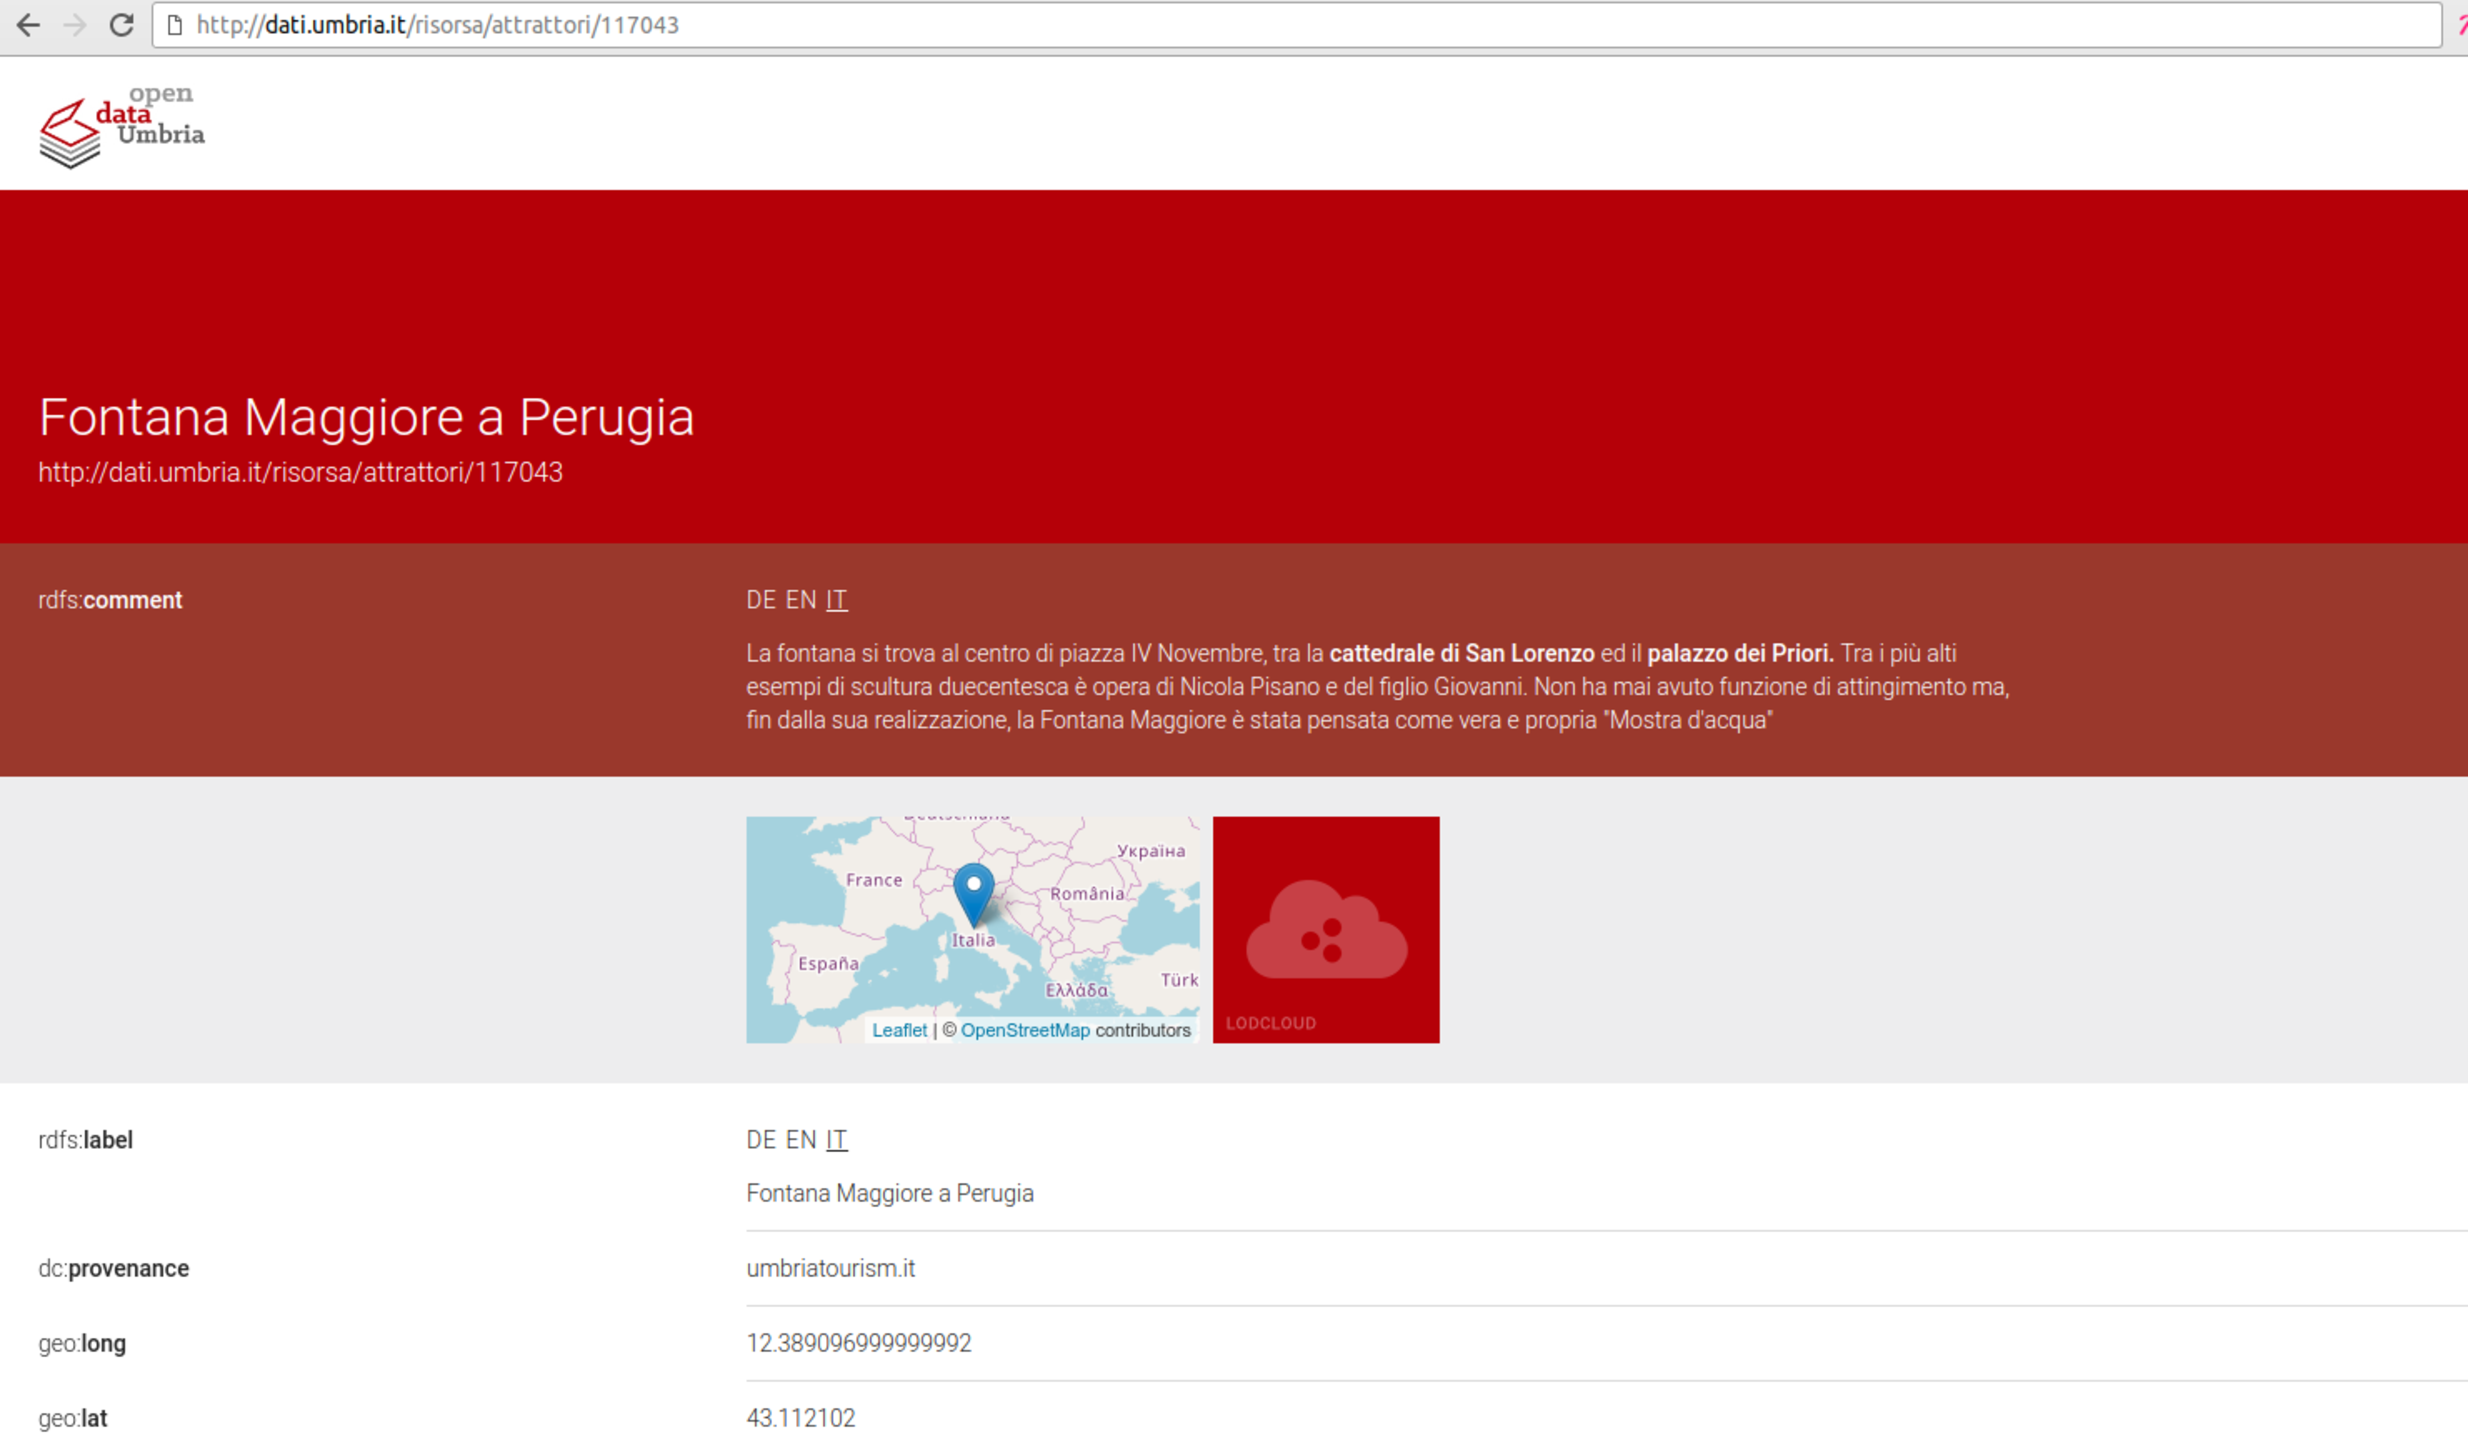
\includegraphics[width=\textwidth]{gfx/fontana_maggiore_view.pdf} } 
	\caption{Vista HTML di un risorsa RDF (LodView)}
	\label{fig:introduction:url_risorsa_rdf}
\end{figure}


\section{DBpedia}
\label{sec:intro:dbpedia}

La metodologia di produzione dei Linked Data descritta in precedenza è predisposta per ricevere in input i soli dati già strutturati. Per capire i grandi limiti che questa restrizione comporta, si pensi alla grande mole di risorse documentali accumulate dalla pubblica amministrazione. Anche al di fuori dell'ambito governativo la situazione è ugualmente problematica, la gran parte delle risorse di ricerca scientifiche ed enciclopediche di natura documentale sono difficili da trattare. A tal proposito, progetti come \textit{DBpedia} sono nati allo scopo di portare in Linked Data la conoscenza memorizzata su risorse enciclopediche.

DBpedia è un progetto nato nel 2007 allo scopo di costruire una base di conoscenza Linked Data a partire dagli articoli del popolare sito Web Wikipedia. Gli articoli di DBpedia contengono la maggior parte delle informazioni nel testo libero, come già detto, difficilmente trattabile. Ma include anche informazioni strutturate come le \textit{infobox} (le tabelle laterali che appaiono in alto a destra in molti articoli e che costituiscono un riepilogo formale dell'articolo), informazioni di categorizzazione, immagini, coordinate geografiche e link ad altri articoli e pagine Web esterne.

Le informazioni vengono estratte maggiormente dalle infobox in maniera automatizzata, utilizzando delle associazioni tra proprietà OWL e voci delle infobox. Tuttavia la gran parte dell'informazione nascosta nella parte più significativa dell'articolo, il contenuto in testo libero, non viene utilizzata.

\subsection{DBpedia Challenge}
\label{sec:intro:dbpedia:challenge}

Il problema di estrarre Linked Data nascosti nel testo libero è di notevole importanza, ma ancora irrisolto. Allo scopo di favorire il progresso in questo tipo di sfida l'organizzazione DBpedia ha organizzato per l'anno 2017 una competizione chiamata \textit{TextExt - DBpedia Open Extraction Challenge} \cite{DBpedia_TextExt}. Con questa competizione la comunità di DBpedia punta a stimolare il mondo della ricerca a scoprire nuove tecniche e sviluppare nuove soluzioni al fine di estrarre conoscenza dai testi degli articoli di Wikipedia.

La competizione offre due diversi tipi di tracce:
\begin{enumerate}
\item \textit{Triples track (Knowledge extraction)} ha come obbiettivo principale quello di estrarre nuovi fatti (triple RDF) dal testo degli articoli di Wikipedia. Questa traccia è valutata nei seguenti termini:
  \begin{itemize}
  \item Quantità dei dati estratti.
  \item Qualità dei dati estratti misurata da:
    \begin{itemize}
    
    \item Correttezza: viene richiesto di far valutare a ciascuno dei partecipanti una certa quantità di triple. Le triple provengono dai vari progetti e vengono combinate nello stesso insieme per fare in modo che un partecipante possa valutare anche i suoi stessi risultati.
    
    \item Idoneità al caso d'uso proposto: si richiede ai partecipanti di fornire uno specifico caso d'uso per cui il modello di estrazione è progettato per ottenere migliori risultati. Migliori sono i fatti relativi allo specifico caso d'uso e maggiormente il progetto viene valutato.
    
    \item Consistenza e concisione: evitare conflitti ed eterogeneità.
    \end{itemize}
	
    \item Tipo di estrazione: oltre ai fatti viene positivamente valutato ogni risultato che riguarda la conoscenza ontologica (nuovi tipi, tassonomie, assiomi e domini e co-domini delle proprietà).
  
  	\item Lingue supportate.
  
  	\item Abilità di mantenere la conformità al formato NIF proposto.

	
  \end{itemize}
  
\item \textit{Annotation track}: ha come obiettivo l'aggiunta di annotazioni NLP al testo libero degli articoli. E' richiesto il formato NIF, un modello per la specifica di proprietà NLP basato su RDF/OWL. E' accettato e positivamente valutato qualsiasi tipo di annotazione utile al fine della prima traccia: lemmi, \textit{POS (Part of Speech)} tag, dipendenze, coreferenza, alberi sintattici, \textit{NER (Named Entity Recognition)}, \textit{NEL (Named Entity Linking)} etc..
\end{enumerate}


TextExt viene annunciato come una competizione che differisce in modo significativo dalle altre sfide nella tecnologia del linguaggio in quanto si propone di essere un challenge in continuo sviluppo nel tempo e non una chiamata unica.





\section{Struttura della tesi}
\label{sec:intro:structure}

Come già accennato, il lavoro di questa tesi è stimolato dal problema ancora aperto dell'estrazione di informazioni strutturate nascoste nei testi liberi. 
L'interesse a questo problema e l'esperienza accumulata nella produzione e utilizzo di Linked Open Data, hanno portato l'autore ad affrontare la sfida proposta da DBpedia (descritta nella sezione precedente \ref{sec:intro:dbpedia:challenge}), proponendo una propria soluzione che viene documentata in questa tesi.

In questo capitolo si è introdotto il concetto di Semantic Web evidenziando le motivazioni che ne hanno determinato la nascita, spiegando come avviene il processo produttivo e l'utilizzo dei Linked Open Data e i limiti attuali. Nel capitolo \ref{sec:literature_review} viene delineato dettagliatamente il problema affrontato e fatta una panoramica dei lavori correlati. Viene spiegata la soluzione proposta nel capitolo \ref{sec:methods} e nel successivo capitolo \ref{sec:results} se ne espongono i risultati prendendo in esame i test effettuati. Nell'ultimo capitolo \ref{sec:conclusion} vengono ipotizzate delle migliorie per il progetto e sviluppi futuri in generale.





% !TEX root = ../my-thesis.tex
%
\chapter{Definizione del problema e lavori correlati}
\label{sec:literature_review}

Lo scopo del lavoro di questa tesi è quello di costruire un sistema software che analizzi testi documentali scritti in linguaggio naturale con l'obbiettivo di estrarre dati in formato RDF (triple) che possano essere aggiunti ai dati di una base di conoscenza.

Questo progetto rientra nell'ambito della \textit{Knowledge Base Construction}.
Il processo di costruzione di una base di conoscenza si compone di due operazioni fondamentali: l'architettura e il popolamento. 

In particolare ci si è concentrati sulla risoluzione del problema del popolamento, denominato convenzionalmente come \textit{KBP (Knowledge Base Population)}, prendendo in oggetto basi di conoscenza già costruite seguendo il modello Linked Data.

Il tema KBP è attualmente oggetto di ricerca come dimostrato dall'impegno del NIST (National Institute of Standards and Technology) nel riproporre, nel convegno annuale TAC\cite{TAC}, un workshop rivolto ad alimentare la ricerca in questo settore. In particolare è di interesse, per il progetto di questa tesi, il task \textit{Slot Filling}, che prevede il popolamento di una base di conoscenza a partire da \textit{entità} e \textit{proprietà} note (Sezione \ref{sec:intro:web_history}).

Il popolamento di basi di dati Linked Data costituisce una specializzazione del problema KBP. I progetti maggiormente impegnati in quest'ambito sono YAGO\cite{Suchanek2007YagoAC} e DBpedia\cite{Lehmann2015DBpediaA}. Quest'ultimo ha contribuito ad incentivare la ricerca in quest'area tematica proponendo nell'anno 2017 la competizione \textit{TextExt - DBpedia Open Extraction Challenge}\cite{DBpedia_TextExt}.

KBP fa parte dell'ambito di ricerca più generico denominato \textit{IE} (Information Extraction), che riguarda l'estrazione di informazioni strutturate da testi in linguaggio naturale.

Nel seguito di questo capitolo vengono descritti i lavori e le tecniche presenti in letteratura che hanno motivato questo progetto.


%Quello della costruzione di basi di conoscenza è un ambito dell'Intelligenza Artificiale studiato già da prima della formulazione del concetto di Web. L'interesse per questo strumento è nato dall'esigenza di strutturare i dati in maniera ben organizzata, facilmente consultabile da tutti e processabile dai computer. La nascita del Semantic Web ha reso possibile per le basi di conoscenza di essere distribuite, collegate e uniformemente strutturate.

%Il requisito delle basi di conoscenza di essere agevolmente consultabili da tutti marca una netta differenza con i database, in cui i dati e le loro relazioni sono noti ai soli tecnici e sono architettati al fine della progettazione del software.
%I documenti testuali, pur raccogliendo conoscenza fruibile a tutti, non soddisfano invece il requisito \textit{machine readable}.
%I database e i contenuti testuali documentali rappresentano la sorgente dati delle basi di conoscenza.

%Un esempio di costruzione di basi di conoscenza a partire da basi di dati è stato già descritto nella sezione \ref{sec:intro:linked_data_production}, mostrando che è un compito già automatizzabile, diffuso (nelle organizzazioni governative) e privo di problemi rilevanti.













\section{Information Extraction}
\label{sec:literature_review:information_extraction}

L'Information Extraction si occupa di identificare le entità presenti in un testo e i fatti asseriti che le riguardano al fine di estrarre informazioni strutturate. Le tecniche utilizzate rientrano nell'ambito di quello che viene chiamato \textit{Natural Language Processing} (\textit{NLP}).

L'estrazione di dati strutturati da testo libero si compone di due sottoproblemi: la scoperta delle menzioni delle \textit{entità} di interesse (\textit{entity mentions}) e l'identificazione delle \textit{relazioni} che le riguardano (\textit{relation mentions})\cite{Grishman2012InformationEC}.

Le menzioni da ricercare sono di tre tipi:
\begin{itemize}
\item \textit{Named Mentions}: menzioni dei nomi delle entità ricercate (es. "Francesco Totti"). 
\item \textit{Pronoun Mentions}: menzioni ad entità tramite pronomi.
\item\textit{Nominal Mentions}: menzioni ad entità di tipo nominale (es. "l'ottavo re di Roma").
\end{itemize}
Le tecniche rivolte al riconoscimento e classificazione del primo tipo di menzioni vengono definite \textit{Named Entities Recognition} (\textit{NER}), mentre per gli altri due tipi si parla di \textit{Coreference Resolution}.

Nell'ambito della NER vengono convenzionalmente definite delle categorie standard. Le più comuni sono \textit{PERSON} per le persone, \textit{GPE} per le entità geografiche e politiche, \textit{ORGANIZATION} per le organizzazioni. Anche le espressioni temporali vengono considerate come categoria della NER (\textit{DATE}). 
Fare NER significa individuare nel testo le named entity e dedurne la categoria di appartenenza.
Ad oggi la tecnica NER è implementata nella maggior parte dei software di NLP ed ha raggiunto risultati accurati sia a livello di precisione che di richiamo.
 

Quello della coreference resolution è un problema ancora aperto, specialmente per le lingue diverse da quella inglese. Questo tipo di tecnica prevede il riconoscimento di riferimenti ad entità che non sono espliciti, ma avvengono tramite quelle che in linguistica vengono definite \textit{anafore}. Tale problema è molto condizionato dalle specificità delle lingue, dal tipo di contesto ed è difficile da valutare. Per queste ragioni non molti software NLP implementano questa funzionalità e se lo fanno è generalmente disponibile in poche lingue ed ha scarsa efficacia.

Il problema dell'identificazione delle menzioni di relazioni riguarda invece la ricerca di predicati o proprietà che associano le entità tra loro. Per le coppie di entità di tipo PERSON, una relazione potrebbe essere quella di essere sposati. Questa relazione può essere espressa in vari modi ed etichettata con annotazioni di diversa provenienza che tuttavia hanno lo stesso valore semantico. Il legame coniugale, ad esempio, può essere rappresentato dall'arbitraria annotazione "essere\_sposati" o da un \textit{frame semantico} o da una proprietà o predicato definito in una tassonomia come la proprietà \textit{dbo:spouse} presente nell'OWL di DBpedia.

Le tecniche che cercano di risolvere questo problema a livello linguistico/semantico rientrano nell'ambito del \textit{semantic role labeling}.
Solitamente queste tecniche sono di apprendimento automatico supervisionato allenato su corpus testuali manualmente annotati con frame semantici come \textit{FrameNet} \cite{FrameNet} o \textit{PropBank}\cite{Kingsbury2002FromTT}.
Nella KBP di Linked Data la relation extraction è di fondamentale importanza. Le relazioni da scoprire sono definite nelle ontologie sotto forma di predicati: la procedura consiste nel collegare (\textit{linking}) caratteristiche di una proposizione testuale (features linguistiche) ad un predicato già definito.

La risoluzione dei problemi precedentemente descritti non può prescindere da una preventiva analisi del testo tramite NLP. Tale analisi prevede vari passaggi sequenziali che estraggono \textit{features} linguistiche utilizzate come input per il passo successivo. Si inizia suddividendo il testo in frasi e si prosegue suddividendo le frasi in \textit{token}. La generazione di token (\textit{tokenization}) ha il compito di tagliare una sequenza di caratteri in segmenti significativi, escludendo alcuni tipi di caratteri non desiderati come i simboli di punteggiatura. Successivamente avviene l'analisi dei \textit{chunk}: blocchi di token che rappresentano parti sintattiche del discorso (\textit{Part of speech}). I vari chunck vengono analizzati con delle regole grammaticali per costruire un albero delle dipendenza sintattiche.

Le features linguistiche prodotte dal processo NLP vengono sfruttate nell'IE per implementare la scoperta e la classificazione delle entità e successivamente, per ogni coppia di entità, per dedurre la relazione corretta. L'intero processo appena descritto è rappresentato nella figura \ref{fig:literature_review:ie} 
%Controllare numero aggiungere vertical space e riquadro

\begin{figure}[htb]
\fbox{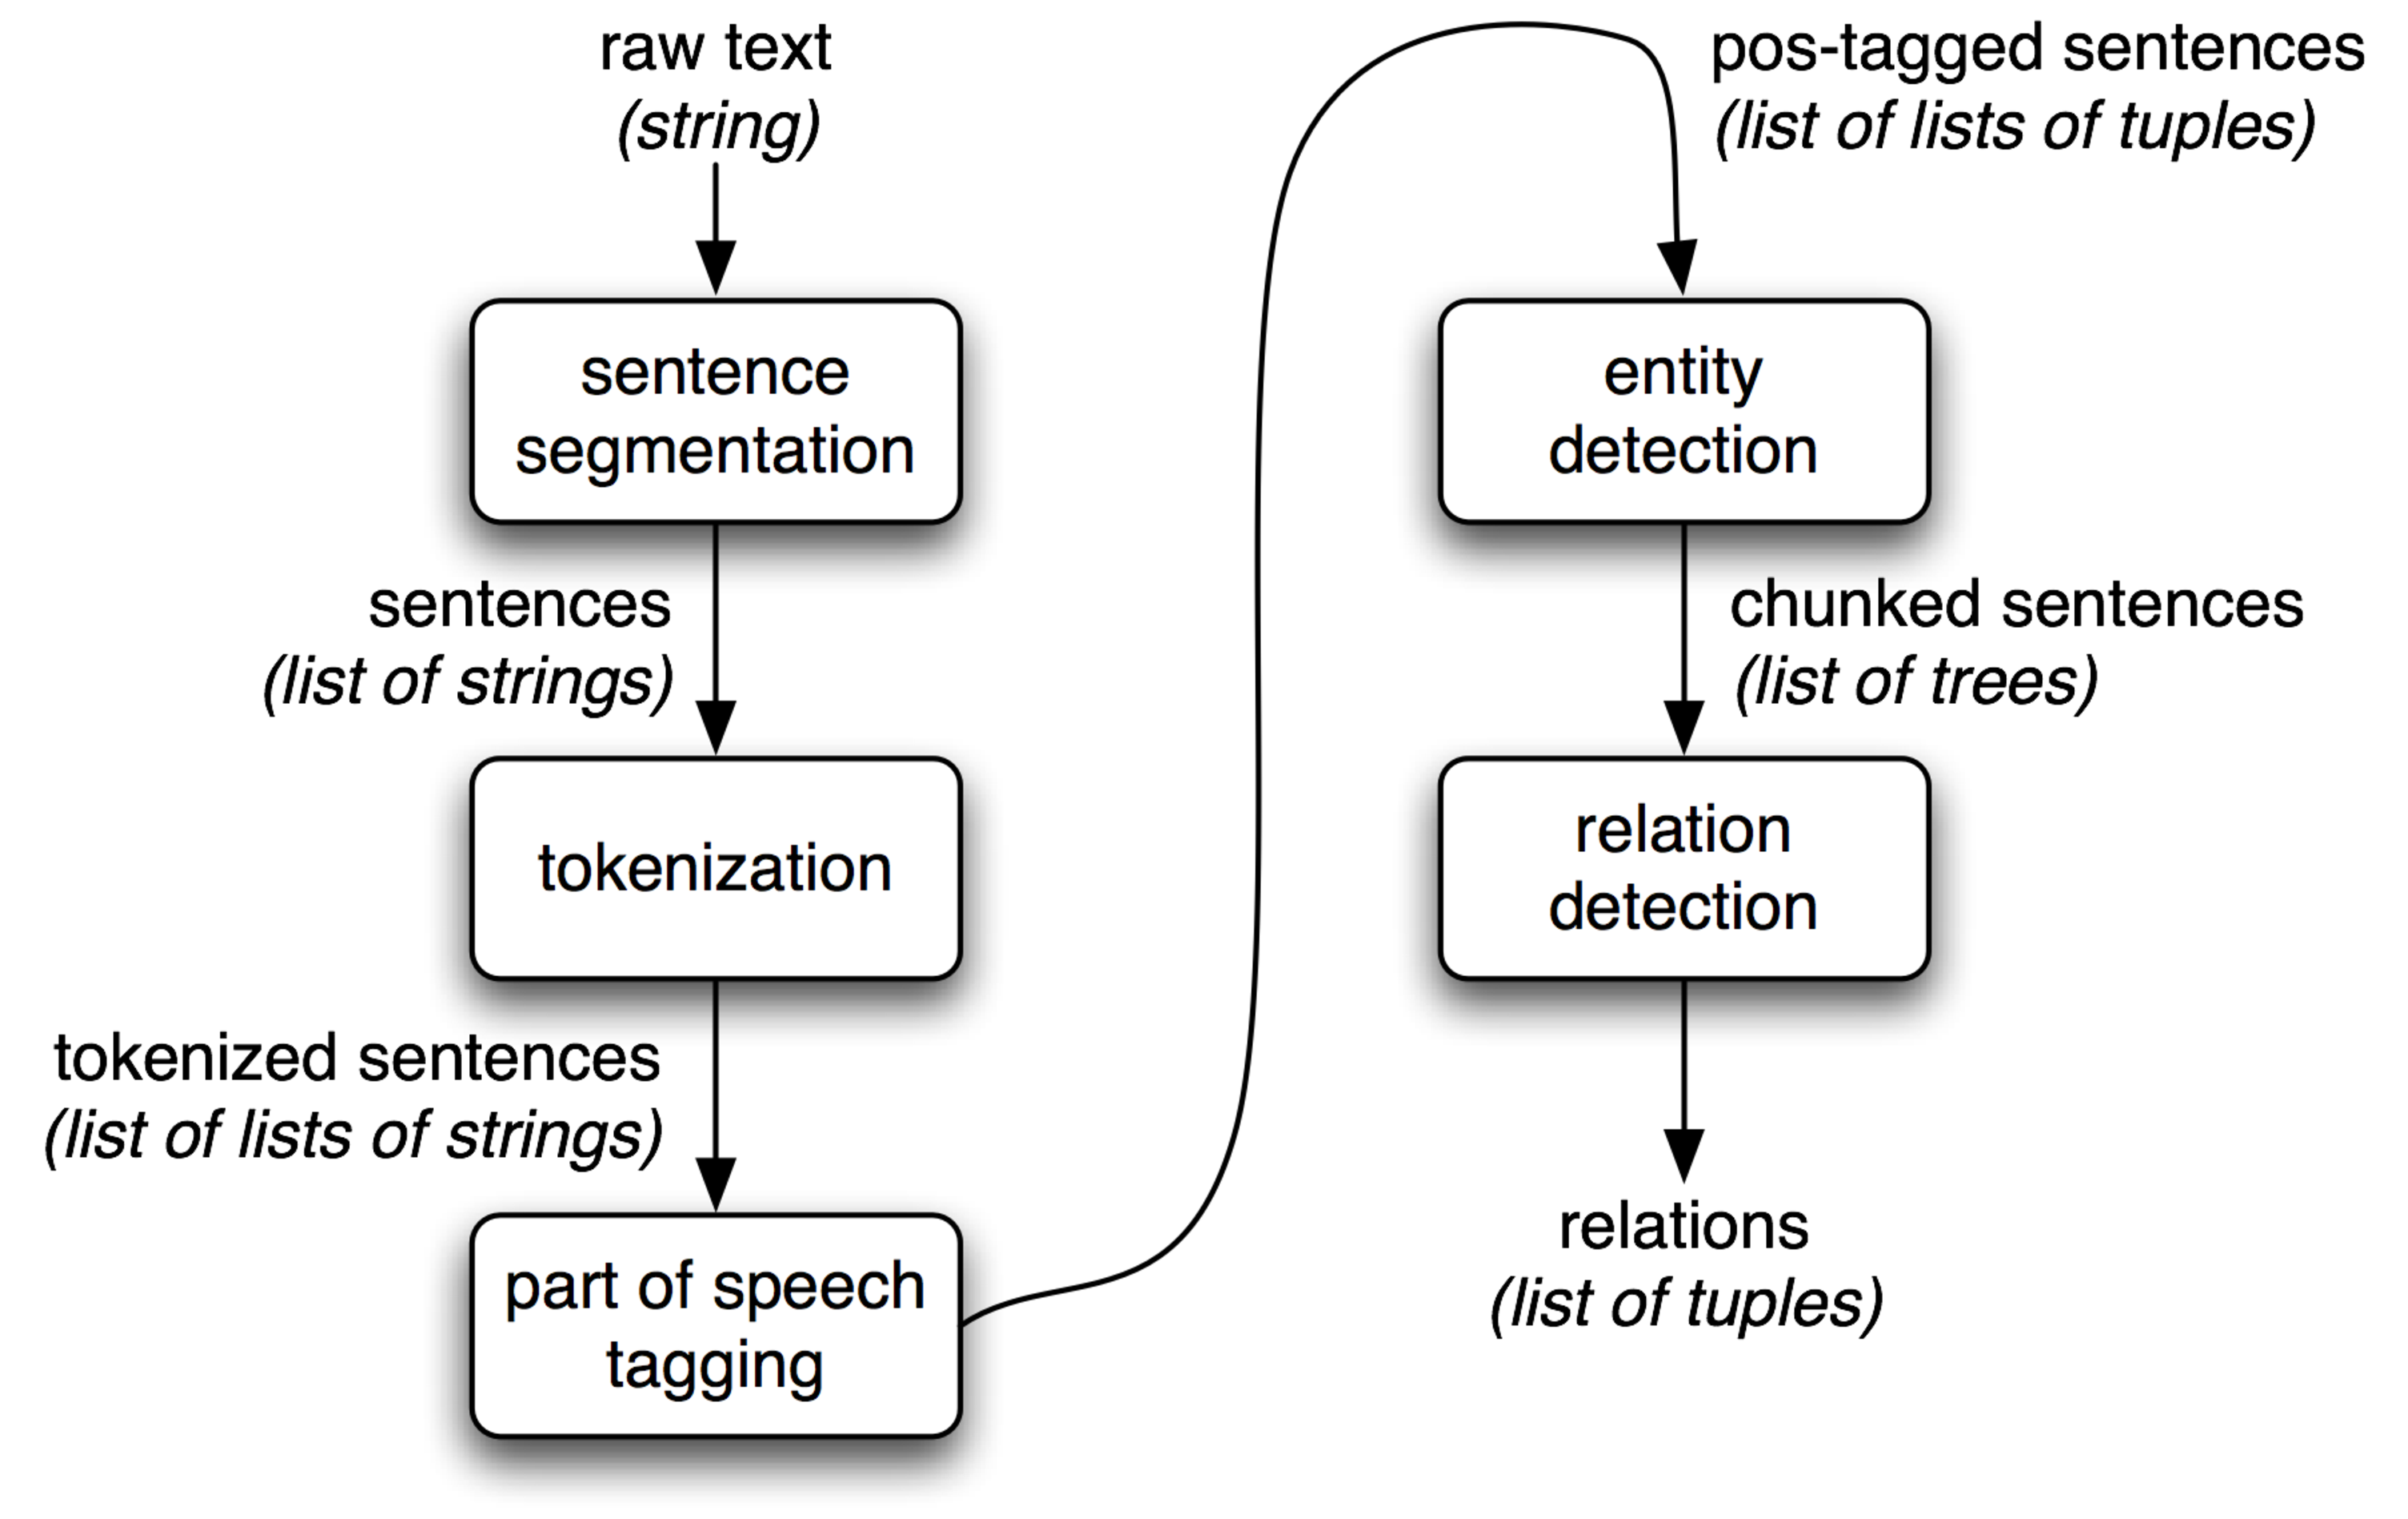
\includegraphics[width=\textwidth]{gfx/ie-architecture.pdf}  }
	\caption{Processo di Information Extraction}
\label{fig:literature_review:ie}
\end{figure}

Le strategie che sfruttano features linguistiche nell'ambito dell'IE sono:
\begin{itemize}
\item Regole programmate a mano.
\item Apprendimento supervisionato in cui tutti i dati di training sono etichettati.
\item Apprendimento non supervisionato in cui non si fa uso di insiemi di training.
\item Apprendimento semi-supervisionato in cui solo una parte dell'insieme di training è etichettato.
\end{itemize}
Le regole programmate a mano, come noto, pur essendo efficienti in casi particolari, si dimostrano inattuabili se il problema da modellare ha un input troppo esteso o dipende da un elevato numero di fattori.

Se da un lato l'apprendimento supervisionato mostra ottimi risultati, dall'altro si rivela attuabile solo se esistono insiemi di training naturalmente etichettati. E' il caso, per esempio, del semantic role labeling usando corpus annotati con semantic frame. L'operazione di etichettare i dati a mano può essere molto dispendiosa in casi come quello della KBP in cui le classificazioni da fare (i diversi tipi di relazioni da scoprire) sono numerose.

I sistemi di apprendimento non supervisionato si basano solamente sulle caratteristiche dell'input e non su dati precedentemente etichettati. Nell'ambito dell'IE non vengono utilizzate frequentemente a causa della scarsa efficienza e della difficoltà nella valutazione dei modelli prodotti. 

In alternativa si usano procedure semi-supervisionate in cui si prende in input un piccolo insieme etichettato (L) ed un altro non etichettato (U). Generalmente l'apprendimento semi-supervisionato si basa sull'avere un classificatore che non solo può classificare nuovi dati, ma può stimare il livello di fiducia nella sua classificazione. Il processo funziona in modo iterativo, aumentando gradualmente l'insieme L e quindi migliorando il classificatore. Ad ogni iterazione, il classificatore viene allenato su L, applicato ad U, generando nuove etichette la cui affidabilità viene valutata. Le nuove etichette con livello di confidenza più alto vengono aggiunte ad L, mentre le altre restano in U. Un limite di questo sistema è il riconoscimento di un'adeguata condizione di terminazione. Per favorire una corretta valutazione delle etichette prodotte viene talvolta sfruttata la tecnica di \textit{Active Learning}, in cui le etichette vengono valutate interattivamente da un agente umano.

Un tipo di apprendimento semi-supervisionato molto particolare e utilizzato in ambito IE è la \textit{Distant Supervision}. Questa tecnica consiste nel costruire un insieme di training interrogando automaticamente una base di conoscenza. Una volta costruito l'insieme di training, si effettua un allenamento e una classificazione in maniera supervisionata. Tecniche di questo tipo, che permettono la classificazione non disponendo di una base di verità (\textit{ground truth}), bensì cercando di approssimarla, rientrano nella categoria definita come \textit{weak supervision}.
Tali tecniche sono soggette alla produzione di etichette con presenza di rumore o con una bassa copertura. A tal proposito, un problema attualmente aperto, è quello di cercare di coniugare i segnali prodotti dall'azione di varie tecniche di questo tipo in un unico risultato \cite{Ratner2017SnorkelFT}.

Citando \citet{Grishman2012InformationEC}, bisogna tenere in mente che, anche se in alcuni casi l'apprendimento completamente automatico batte i migliori sistemi programmati a mano, in molti casi la congiunzione di machine learning e regole esplicitamente programmate è difficile da superare. Il progetto di questa tesi si ispira a questa idea, prevedendo infatti un approccio che affianca regole programmate in maniera esplicita con strumenti di classificazione semi-supervisionata come la distant supervision.

\subsection{Distant Supervision}
\label{sec:literature_review:information_extraction:distant_supervision}
Un tipo di apprendimento semi-supervisionato che ha ricevuto molta attenzione nella letteratura riguardante IE, ed in particolare in KBP, è quello denominato \textit{\textbf{Distant Supervision}}. Questa tecnica si basa sull'assunzione di poter fare affidamento su una base di conoscenza contenente istanze della relazione d'interesse e su un corpus di testo di grandi dimensioni contenente menzioni a molte delle istanze della base di conoscenza. Usando questa combinazione si possono costruire automaticamente insiemi di istanze positive e negative per la classificazione di relazioni. 

Questo approccio è stato descritto come "learning from weakly labeled data" [CK99] e più recentemente soprannominato \textit{Distant Supervision} \cite{Mintz2009DistantSF}.
Il nome deriva dal fatto che la base di conoscenza fornisce supervisione, ma non tramite annotazione diretta dei dati di testo. 

Nell'etichettamento (\textit{labeling}) dell'insieme di allenamento si prendono le istanze [Soggetto, Oggetto] della relazione nella base di conoscenza e si raccolgono tutte le proposizioni nel corpus testuale contenenti entrambe le menzioni alle due entità. Tali segmenti di testo diventano gli esempi etichettati positivamente, le restanti proposizioni vengono etichettate come negative. L'insieme prodotto viene poi utilizzato per allenare ed applicare un classificatore allo stesso modo di un approccio supervisionato.

La distant supervision è in grado di produrre una grande quantità di dati di training che potrebbero però essere rumorosi. Questa tecnica presenta i seguenti problemi:
\begin{itemize}
\item per una coppia di entità potrebbero sussistere più tipi di relazione. Questa caratteristica deriva in una produzione di etichette di training erroneamente positive e una conseguente generazione di classificazioni \textit{false positive}.
\item La base di conoscenza può essere incompleta. In tal caso molte frasi, che dovrebbero essere etichettate come positive, vengono scartate, implicando un numero elevato di \textit{falsi negativi}.
\item Il risultato finale è influenzato dall'accuratezza dell'\textit{entity linking} tra la menzione testuale e il valore dell'entità nella base di conoscenza (Es. collegare la menzione "Plant" all'entità "Robert Plant"). Tale operazione può essere soggetta ad \textit{overfit}, scartando menzioni valide o \textit{underfit} collegando erroneamente menzioni a entità. 
\end{itemize}




\section{Knowledge Base Population}
\label{sec:literature_review:kbp}

Con il termine \textit{KBP} (\textit{Knowledge Base Population}) ci si riferisce al problema di:
\begin{enumerate}
\item estrarre dal testo libero nuove informazioni riguardanti entità della KB;
\item strutturare le informazioni estratte secondo il modello della KB;
\item aggiungere le nuove informazioni strutturate alla KB.
\end{enumerate}

L'impegno nella risoluzione del problema di KBP è stato ripetutamente alimentato e rilanciato dal \textit{NIST} (\textit{National Institute of Standards and Technology}) nella conferenza annuale \textit{TAC} (\textit{Text Analysis Conference}). TAC è composta
da una serie di seminari organizzati per incoraggiare la ricerca nell'elaborazione del linguaggio naturale (NLP) e lo sviluppo delle relative applicazioni\cite{TAC}. TAC prevede anche un insieme di competizioni note come \textit{tracks}, ognuna delle quali si concentra su un particolare sottoproblema di NLP, come la Knowledge Base Population.

Questa competizione è stata avviata anche nell'ultima conferenza del 2017 e si compone di quattro task:
\begin{enumerate}
\item \textit{Entity Discovery and Linking (EDL)}: identificare menzioni di entità (\textit{entity mentions}) e collegarle al nodo corrispondente nella base di conoscenza.
\item \textit{Slot Filling}: dato un insieme di proprietà (\textit{slots}) trovare il valore specifico per le varie entità. 
\item \textit{Event}: estrarre dal testo libero informazioni riguardanti eventi.
\item \textit{Belief and Sentiment}: individuare opinioni e sentimenti di entità nei confronti di altre entità, relazioni o eventi.
\end{enumerate}

Il lavoro di questa tesi punta a dare un contributo esclusivamente ai primi due task, con la particolarità che le entità e gli "slot" presi in considerazione sono le entità e i predicati del mondo Linked Data.

Fare KBP su basi di conoscenza Linked Data significa estrarre proposizioni dal testo in lingua naturale che siano rappresentabili come un'asserzione (s,p,o) RDF.
Più precisamente Linked Data KBP (denominata d'ora in poi come LDKBP) è il processo che prevede di:
\begin{enumerate}
\item individuare nel testo le menzioni di entità e la loro categoria (NER),
\item collegarle le named entity estratte alle corrispondenti entità RDF appartenenti alla base di conoscenza Linked Data (entity linking), 
\item identificare le relazioni che hanno come soggetto o oggetto le entità estratte (relation extraction),
\item collegare i predicati dei vocabolari OWL, usati nella KB e trattati come input, con le relazioni estratte (\textit{relation linking}), 
\item formare delle proposizioni RDF, da aggiungere alla base di conoscenza con le entità e i predicati estratti (slot filling o più nello specifico \textit{triples extraction}).
\end{enumerate}

Il processo LDKBP è composto da due input: il testo libero da analizzare e le proprietà Linked Data da ricercare.
L'input di tipo testuale non ha particolari requisiti o limitazioni ed è di conseguenza potenzialmente molto vasto.
Le entità e i predicati Linked Data hanno ormai raggiunto una larga definizione e rispecchiano quasi ogni entità o proprietà della realtà a noi conosciuta. Queste caratteristiche dimensionali dell'input comportano delle limitazioni nelle strategie adottabili per l'elaborazione. Le tecniche adottate sono quindi principalmente di apprendimento automatico o in alcuni casi impiegano delle regole esplicitamente programmate che sfruttano strutture deboli ricorrenti nel testo libero.

Due esempi di LDKBP che sfruttano strutture ricorrenti nel testo esaminato sono fornite da YAGO\cite{Suchanek2007YagoAC} e DBpedia\cite{Lehmann2015DBpediaA}. I due progetti hanno come corpus Wikipedia, i cui articoli consistono principalmente di testo libero, ma comprendono anche vari tipi di informazioni strutturate sotto forma di markup. Tali informazioni includono infobox, informazioni di categorizzazione, immagini, coordinate geografiche, collegamenti a pagine Web esterne, pagine di disambiguazione e collegamenti ad altre risorse o a risorse equivalenti in altre lingue. I framework dietro DBpedia e YAGO estraggono informazioni strutturate e le trasformano in dati di una base di conoscenza di dominio generico. Per potersi avvalere di queste informazioni sono state costruite delle apposite ontologie OWL con le quali mappare a mano i diversi tipi di strutture presenti. Un progetto analogo ai precedenti due, ma attualmente dismesso, è \textit{Freebase}.

Come già accennato in precedenza, per quanto riguarda l'utilizzo di machine learning in ambito di IE, si fa uso, in particolare nella letteratura più recente, della tecnica di distant supervision. 

Questa tecnica prevede l'utilizzo delle istanze di una base di conoscenza per etichettare automaticamente un insieme di training per un classificatore. Nella fase di labeling si prendono le istanze [Soggetto, Oggetto] della relazione nella base di conoscenza e si raccolgono tutte le proposizioni nel corpus testuale contenenti entrambe le menzioni alle due entità. Il testo estratto diventa parte dell'insieme di training per il classificatore.

Un iniziale approccio di questo tipo si è avuto con \citet{Craven1999ConstructingBK} nella costruzione di una base di conoscenza in ambito biologico di localizzazione subcellulare. In tale lavoro sono stati usati come input testuali i documenti del database bibliografico \textit{MEDLINE} e come risorsa per la distant supervision il database \textit{Yeast Protein Database}. Successivamente \citet{Mintz2009DistantSF} hanno usato Freebase come base di conoscenza (considerando le 102 proprietà più ricorrenti), mentre Wikipedia è stata utilizzata come fonte di testo. E' stato utilizzato un insieme di features linguistiche per allenare un classificatore in grado di avere alta precisione. Il modello è stato valutato a mano considerando le 100 o 1000 istanze estratte di maggior confidenza per ciascuna relazione dimostrando una misura F1 tra il 67\% e il 69\%.

Successivamente \citet{Nguyen2011EndtoEndRE} hanno utilizzato nel loro lavoro un sistema di valutazione più adeguato annotando 200 documenti con 52 relazioni e misurando un valore \textit{F1} pari al 67\%.

Recentemente il progetto di \citet{Cannaviccio2016AccurateFH} basato su distant supervision di articoli di Wikipedia con il database \textit{Freebase} si è posizionato al primo posto nella competizione TextExt di DBpedia. La particolarità di questo progetto è quella di avere un supporto multi-lingua e di discriminare le relazioni ,non in base alle generiche features linguistiche, ma in funzione delle cosidette \textit{typed phrase}: segmenti testuali che identificano le proprietà della base di conoscenza da popolare. Purtroppo non si conoscono dettagli sulle prestazioni di questo progetto.

\subsection{Data Programming in Snorkel}
\label{sec:literature_review:data_programming}

La distant supervision è una tecnica che permette un approccio di machine learning debolmente supervisionato creando insiemi di training quando non sono naturalmente disponibili, ma è soggetta a problemi di: incompletezza della base di conoscenza, difficoltà nell'entity linking, relazioni multiple per le entità. Tali problemi introducono rumore e bassa copertura dei dati etichettati che si riflette sulla classificazione finale.
Il paradigma \textit{data programming} \cite{Ratner2016DataPC, Ehrenberg2016DataPW,Bach2017LearningTS} è stato ideato per costruire automaticamente insiemi di allenamento, limitando la presenza di rumore e senza avere accesso ad una base di verità.
 
La tecnica di data programming è stata teorizzata, implementata e rilasciata pubblicamente dalla \textit{Stanford University} nei progetti \textit{DeepDive}\cite{Niu2012DeepDiveWK} e nella sua evoluzione \textit{Snorke}l\cite{Ratner2017SnorkelFT}. Lo sviluppo del primo progetto è stato dismesso in favore del secondo, per tale ragione ci si riferirà nel seguito della tesi al progetto Snorkel.

Snorkel viene presentato come il primo sistema "end-to-end" in grado di addestrare modelli di machine learning allo stato dell'arte senza disporre di dati etichettati manualmente. Il testo libero viene etichettato automaticamente da quelle che vengono chiamate \textit{labeling functions}: funzioni programmate, che esprimono euristiche arbitrarie e che possono avere precisione e correlazione sconosciuta. 
La tecnica di data programming permette di raffinare i segnali prodotti dalle varie labeling functions in base a quanto esse sono concordanti o discordanti, producendo un insieme etichettato con bassa presenza di rumore.

Le varie labeling function sono fonti di weak supervision e sono dei seguenti tipi:
\begin{itemize}
\item \textit{Distant Supervision}.
\item \textit{Pattern-based}: euristiche basate su un modello fornito da un esperto del dominio. 
\item \textit{Weak classifier}: classificatori insufficienti per l'intero problema, con una copertura limitata, rumore o allenati su dataset differenti.
\item \textit{Crowdsourcing}: etichette generate a mano da utenti non esperti e imprecisi.
\end{itemize}

Nella loro forma più generale, le labeling function sono semplicemente snippet di codice scritti in Python che accettano in input un oggetto \textit{Candidato} e restituiscono in output un'etichetta positiva o negativa o si astengono. Un oggetto candidato è un segmento di testo delimitato da due token (\textit{Span}) filtrato dal resto del corpus in base a delle features arbitrarie fondamentali che lo rendono plausibilmente adatto ad essere considerato come esempio da etichettare. Si consideri come esempio la relazione "essere sposato" per cui sono candidati solamente i segmenti di testo delimitati da due named entities del tipo PERSON. 

Nell'approccio di data programming, le varie funzioni di labeling descrivono implicitamente un modello generativo. Avendo dati \textit{x}, con etichette da prevedere \textit{y}, in un approccio discriminativo si modella direttamente \textit{P (y | x)}, mentre in un approccio generativo si modella \textit{P (x, y) = P (x | y) P (y)}. Nel caso specifico si modella un processo di formazione delle etichette dell'insieme \textit{P (L, y)}, dove \textit{L} sono le etichette generate dalle labeling functions per gli oggetti \textit{x}. Costruendo un modello generativo e stimando direttamente \textit{P (L | y)}, si apprende essenzialmente l'accuratezza relativa delle funzioni di labeling in base a come si sovrappongono o sono in conflitto. 

L'output di Snorkel è un insieme di \textit{probabilistic labels}, ovvero etichette con una probabilità marginale di attendibilità, che possono essere usate per allenare una larga varietà di modelli discriminativi di machine learning, come ad esempio i popolari modelli di deep learning.
Mentre il modello generativo è essenzialmente una combinazione ripesata delle labeling function fornite dall'utente, che tendono ad essere precise ma con una bassa copertura, i modelli discriminativi moderni possono conservare questa precisione incrementandone la copertura. 

Snorkel comprende funzionalità "built-in" o integrate che rendono applicabile l'intero processo di classificazione a partire dal solo corpus testuale non etichettato. Le fasi fondamentali del processo sono:
\begin{enumerate}
\item Parsing del corpus testuale con tool di NLP integrati e integrabili.
\item Estrazione degli oggetti candidati in base alle features NLP ricavate nella fase precedente.
\item Definizione e applicazione delle labeling function agli oggetti candidati.
\item Allenamento del modello generativo (built-in) con i segnali prodotti dalle labeling functions.
\item Classificazione degli oggetti candidati con il modello generativo, producendo etichette probabilistiche.
\item Allenamento di modelli discriminativi (integrati o integrabili) a partire dalle etichette probabilistiche.
\end{enumerate}
Per predire nuove etichette da esempi non conosciuti si applica nuovamente il parsing NLP, si verifica che si tratti di un oggetto candidato e si usa il classificatore discriminativo. Tra le librerie integrate in Snorkel troviamo \textit{Spacy} e \textit{CoreNLP} per il parsing e \textit{TensorFlow} per il machine learning. Le API fornite da Snorkel consentono un utilizzo semplificato ad alto livello di tali librerie.

La valutazione di Snorkel attribuisce due risultati principali:
\begin{enumerate}
\item Superamento dei risultati ottenuti con le singole tecniche di weak supervision. In particolare è stato valutato che la tecnica più popolare di weak supervision, la distant supervision, può essere superata del 132\%.
\item Creazione di un nuovo paradigma di interazione per la costruzione di insiemi etichettati. E' stato dimostrato empiricamente, in un workshop della durata di due giorni, come utenti possano imparare in così breve tempo a produrre labeling function che ottengono etichette con accuratezza da subito in linea o addirittura superiore a quelle prodotte manualmente in settimane o mesi di lavoro.
\end{enumerate}

I rilevamenti alla base di questi risultati sono stati effettuati nella produzione di modelli per la classificazioni in quattro ambiti diversi: 
\begin{enumerate}
\item \textit{Chem}: estrazione di relazioni tra reagenti chimici e prodotti di reazione negli abstract di PubMed.
\item \textit{EHR}: estrazione di informazioni strutturate Biomediche da referti di pazienti ospedalieri.
\item \textit{CDR}: estrazione dagli abstract di PubMed di collegamenti causali tra sostanze chimiche e malattie.
\item \textit{Spouse}: identificazione di menzioni testuali della relazione coniugale da articoli giornalistici.
\end{enumerate}

\begin{figure}[htb]
	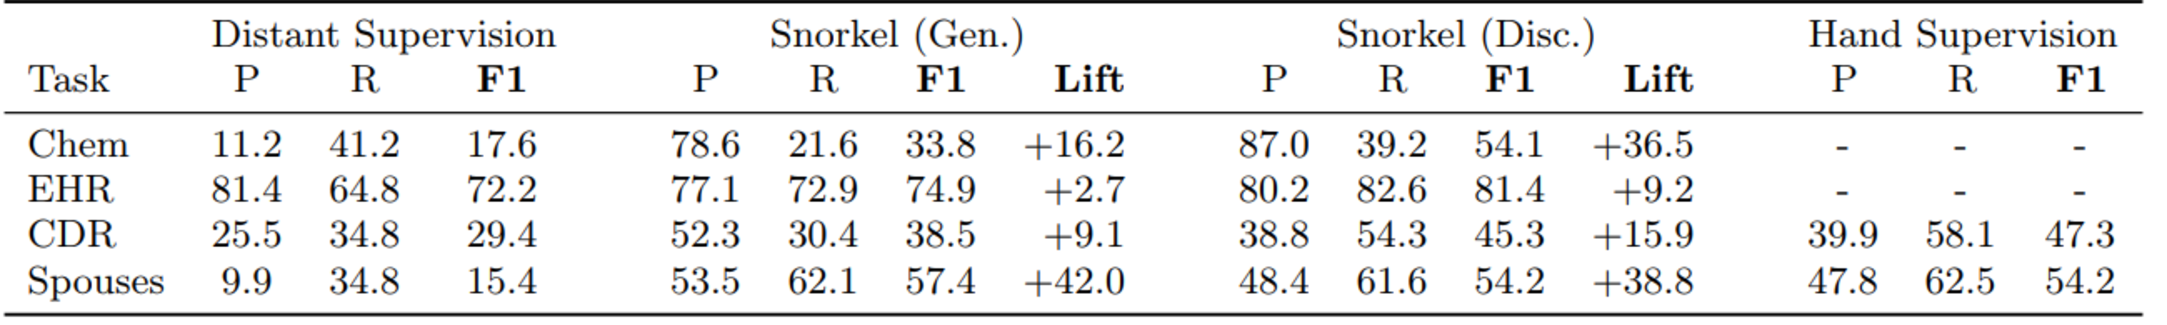
\includegraphics[width=\textwidth]{gfx/snorkel_eval.pdf}  
	\caption{\textit{Valutazione di task di estrazione di informazione dal testo.}}
	\label{fig:literature_review:snorkel_eval}
\end{figure}

I modelli generativi e discriminativi prodotti con Snorkel conseguono risultati migliori della distant supervision e mediamente equivalenti all'etichettamento a mano. Il confronto è stato misurato in termini di precisione \textit{P}, richiamo \textit{R} e media armonica delle due \textit{F1} (Fig. \ref{fig:literature_review:snorkel_eval}).

Il modello discriminativo utilizzato è di tipo \textit{Bidirectional Long Short Term Memory Network} (\textit{Bi-LSTM}) che ha dimostrato risultati allo stato dell'arte nella classificazione di input testuali in ben 22 lingue \cite{DBLP:journals/corr/PlankSG16}.

Al fine del lavoro di questa tesi è stato particolarmente indicativo il risultato raggiunto dal progetto Spouse. In tale caso le labeling functions usate sono state: distant supervision sui dati di DBpedia, modellazione di regole basate su parole chiave e pattern testuali, crowdsourcing. Questa relazione, essendo di dominio generico, è affine alle relazioni presenti in una base di conoscenza Linked Data. In funzione del risultato raggiunto da questo progetto, è lecito domandarsi se tale approccio potrebbe essere applicato al processo di LDKBP, utilizzando la distant supervision come labeling functions di default, ed ottimizzare localmente i risultati per ciascun predicato con labeling functions specifiche e con labeling functions generiche che sfruttano delle parole chiave specifiche. 










%\cite{Palomares2016WikipediaKG} \cite{Bach2017LearningTS}





%Crowdsourcing \cite{FossatiKBP}


%NLP \cite{Etzioni2004WebscaleIE}

%MINTZ The intuition ofdistant supervision is that any sentence that con-tains a pair of entities that participate in a knownFreebase relation is likely to express that relationin some way.  Since there may be many sentencescontaining a given entity pair, we can extract verylarge numbers of (potentially noisy) features thatare combined in a logistic regression classifier. Because our algorithmcan use large amounts of unlabeled data, a pair ofentities may occur multiple times in the test set.For each pair of entities, we aggregate the featuresfrom  the  many  different  sentences  in  which  thatpair appeared into a single feature vector, allowingus to provide our classifier with more information,resulting in more accurate labels. Except for the unsupervised algorithms discussedabove,  previous  supervised  or  bootstrapping  approaches to relation extraction have typically re-lied on relatively small datasets, or on only a smallnumber of distinct relations. Approaches based onWordNet have often only looked at the hypernym(is-a) or meronym (part-of) relation (Girju et al.,2003; Snow et al., 2005), while those based on theACE program (Doddington et al., 2004) have beenrestricted in their evaluation to a small number ofrelation instances and corpora of less than a mil-lion words.Hearst (1992)used a small number of regular expressions overwords and part-of-speech tags to find examples ofthe hypernym relation.  The use of these patternshas been widely replicated in successful systems,for example by Etzioni et al. (2005).The distant supervision assumption is that if twoentities participate in a relation, any sentence thatcontain those two entities might express that rela-tion.   Because  any  individual  sentence  may  givean incorrect cue, our algorithm trains a multiclasslogistic regression classifier, learning weights foreach  noisy  feature.   In  training,  the  features  foridentical  tuples  (relation,  entity1,  entity2)  fromdifferent sentences are combined, creating a richerfeature vector. In the testing step, entities are again identifiedusing  the  named  entity  tagger.   This  time,  everypair of entities appearing together in a sentence isconsidered a potential relation instance, and when-ever those entities appear together, features are ex-tracted on the sentence and added to a feature vec-tor for that entity pair.  For example, if a pair ofentities occurs in 10 sentences in the test set, andeach sentence has 3 features extracted from it, theentity pair will have 30 associated features.  Eachentity pair in each sentence in the test corpus is runthrough feature extraction, and the regression clas-sifier predicts a relation name for each entity pairbased on the features from all of the sentences inwhich it appeared. Consider  thelocation-containsrelation,  imag-ining  that  in  Freebase  we  had  two  instances  ofthis  relation:〈Virginia, Richmond〉and〈France, Nantes〉.   As we encountered sen-tences like ‘Richmond, the capital of Virginia’ and‘Henry’s Edict of Nantes helped the Protestants ofFrance’ we would extract features from these sen-tences.  Some features would be very useful, suchas the features from the Richmond sentence, andsome  would  be  less  useful,  like  those  from  theNantes  sentence.   In  testing,  if  we  came  acrossa  sentence  like  ‘Vienna,  the  capital  of  Austria’,one or more of its features would match those ofthe  Richmond  sentence,  providing  evidence  that〈Austria, Vienna〉belongs  to  thelocation-containsrelation. Our system needs negative training data for thepurposes  of  constructing  the  classifier.   Towardsthis  end,  we  build  a  feature  vector  in  the  train-ing phase for an ‘unrelated’ relation by randomlyselecting  entity  pairs  that  do  not  appear  in  anyFreebase relation and extracting features for them.While it is possible that some of these entity pairs are in fact related but are wrongly omitted fromthe Freebase data, we expect that on average thesefalse negatives will have a small effect on the per-formance of the classifier.   For performance rea-sons, we randomly sample 1% of such entity pairsfor use as negative training examples. By contrast,in the actual test data, 98.7% of the entity pairs weextract do not possess any of the top 102 relationswe consider in Freebase.We  use  a  multi-class  logistic  classifier  opti-mized  using  L-BFGS  with  Gaussian  regulariza-tion.   Our  classifier  takes  as  input  an  entity  pairand a feature vector, and returns a relation nameand a confidence score based on the probability ofthe entity pair belonging to that relation. Once allof the entity pairs discovered during testing havebeen classified, they can be ranked by confidencescore  and  used  to  generate  a  list  of  thenmostlikely new relation instances.

%Distan supervision \cite{Exner2012EntityEF} \cite{Roth2015EffectiveDS} \cite{Mintz2009DistantSF} \cite{Aprosio2013ExtendingTC} \cite{Cannaviccio2016AccurateFH} \cite{Angeli2014CombiningDA}

%TAC \cite{Surdeanu2013OverviewOT}

%TAC E DEEPDIVE \cite{Angeli2014Stanfords2S} \cite{Wu2017FonduerKB}







%The input to a KBC system is a collection of documents. The output of the system is a relational database containing facts extracted from the input and stored in an appropriate schema. To describe the KBC process, we adopt the standard terminology from the KBC community2. There are four types of objects that play integral roles in KBC systems: (1) entities, (2) relations, (3) mentions of entities, and (4) relations mentions.

%An entity e in a knowledge base corresponds to a distinct real-world person, place, or object. Entities in a knowledge base can be grouped in different entity types T1,T2,…,Tn. Entities in a knowledge base participate in relationships. A relationship between n entities is represented as an n-ary relation R(e1,e2,…,en) and is described by a schema SR(T1,T2,…,Tn) where ei∈Ti. A mention m is a span of text that refers to an entity. KBC systems typically assume that all mentions of entities in a document have a corresponding span of text that refers to them. A relation mention candidate is a particular n-ary tuple c=(m1,m2,…,mn) that represents an instance of a relation R(e1,e2,…,en) in a document. If a candidate is classified as true, it is called a relation mention, rR.














% !TEX root = ../my-thesis.tex
%
\chapter{Architettura della soluzione}
\label{sec:methods}


Il lavoro di questa tesi si basa sull'intuizione che i risultati raggiunti nell'ambito della KBP mediante \textit{Distant Supervision} (Sez. \ref{sec:literature_review:information_extraction:distant_supervision}), gli sviluppi introdotti dalla nuova tecnica di \textit{Data Programming} (Sez. \ref{sec:literature_review:data_programming}) e l'efficienza dimostrata dalle \textit{Bidirectional Long Short Term Memory Network} (\textit{Bi-LSTM}) (Sez. \ref{sec:methods:training}) con input sequenziali come il testo libero, possano essere combinati per ottenere risultati allo stato dell'arte nel popolamento di basi di conoscenza Linked Data. 
In particolare il fine è quello di dare una dimostrazione empirica di come una base di conoscenza Linked Data come DBpedia possa essere popolata con nuove triple, composte da predicati già definiti in un'ontologia OWL (DBpedia Ontology), analizzando testi enciclopedici scritti in linguaggio naturale (Wikipedia) e sfruttando l'insieme di triple già esistenti (distant supervision) ed euristiche specifiche (weak supervision) per costruire un insieme di frasi automaticamente etichettate utilizzato per allenare un classificatore di tipo Bi-LSTM.

La tecnica di data programming viene implementata nel progetto Snorkel di cui si fa uso in questo progetto. Grazie a Snorkel è possibile gestire l'intero processo di classificazione a partire dal parsing del corpus fino all'allenamento supervisionato di un classificatore. Il processo viene trattato come un problema di classificazione binaria in cui per un segmento di testo si deve valutare se è adatto o meno a rappresentare una relazione Linked Data. Le triple vengono estratte dalle sole proposizioni testuali classificate positivamente.

Vista la totale indisponibilità di basi di verità etichettate naturalmente, Snorkel ne consente la produzione automatica con varie tecniche di weak supervision implementate dalle \textit{labeling functions}. La distant supervision, la labeling function su cui si ripone maggiore affidamento in questo lavoro, viene potenziata dall'utilizzo di altre funzioni di labeling specifiche.
Con la definizione di semplici labeling functions basate su parole chiave si prevede di aumentare la copertura della distant supervision e limitarne gli errori. In tal caso si raggiungerebbe un risultato pratico importante: l'estrazione di triple potrebbe essere favorita dall'uso di liste di parole chiave la cui produzione può essere fatta manualmente "a basso costo" o automaticamente, instaurando un processo di estrazione iterativamente perfezionabile nel tempo.

Il corpus testuale utilizzato è in lingua Inglese, ma è potenzialmente estendibile a qualsiasi linguaggio naturale supportato dal parser NLP che si decide di utilizzare.

Nel progetto viene impiegata come fonte dati per la distant supervision la stessa base di conoscenza che si vuole popolare: DBpedia. Il punto di accesso per effettuarne l'interrogazione è lo SPARQL Endpoint. Il linguaggio SPARQL viene impiegato sia per il reperimento dei dati campione, che per inferire metadati di interesse sui predicati presi in esame. 

Le etichette prodotte dalle varie labeling function vengono analizzate statisticamente da un algoritmo generativo che ne restituisce le probabilità marginali che vengono a loro volta sfruttate per l'allenamento di un classificatore discriminativo.

Il classificatore ottenuto può essere utilizzato per processare nuovo testo e riconoscere le menzioni testuali dalle quali estrarre delle nuove triple.

Il task di LDKBP si compone di un insieme potenzialmente molto vasto di predicati OWL. Per tale ragione si è progettato un sistema con una struttura \textit{pipeline} adatto ad essere facilmente configurato e ripetutamente eseguito.

\begin{figure}[htb]
	\fbox{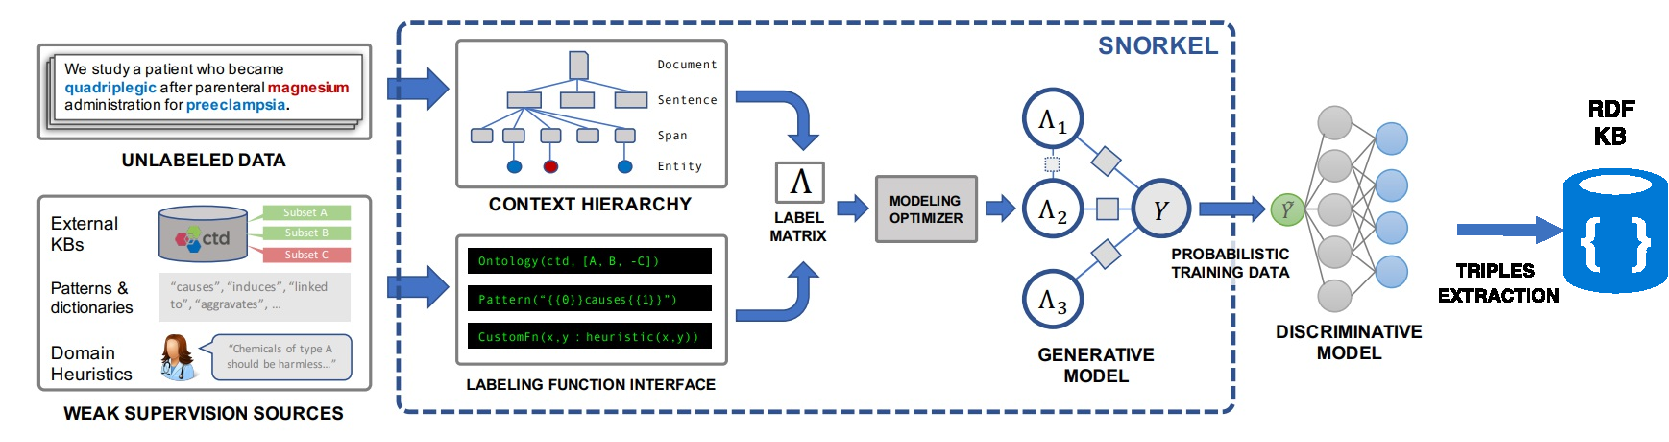
\includegraphics[width=\textwidth]{gfx/sentimantic_diagram.pdf} }
	\caption{Diagramma del progetto.}
	\label{fig:methods:project_diagram}
\end{figure}

Nel corso di questo capitolo si descrive l'ambiente, la configurazione e il processo di funzionamento della pipeline (Fig. \ref{fig:methods:project_diagram}) che si compone dei seguenti passi fondamentali:

\begin{itemize}

\item parsing NLP del corpus Wikipedia: per ogni frase rilevata si memorizzano features testuali (Sez. \ref{sec:methods:text_extraction} e \ref{sec:methods:parsing_nlp});

\item inferenza dei tipi di Named Entity che caratterizzano \textit{dominio} e \textit{range} di ogni predicato in input (Sez. \ref{sec:methods:candidate_inference});

\item etichettamento delle frasi candidate con labeling function  (Sez. \ref{sec:methods:labelling});

\item ottimizzazione dell'insieme etichettato e training del modello di classificazione (Sez. \ref{sec:methods:training});

\item estrazione delle triple dal testo classificato positivamente (Sez. \ref{sec:methods:triples_extraction}).
\end{itemize} 















\section{Configurazione e Ambiente}
\label{sec:methods:config}
Il progetto è strutturato sotto forma di pipeline che ha come input un file di configurazione che descrive:
\begin{itemize}
\item l'URI del corpus testuale;
\item l'URL dello SPARQL Endpoint della base di conoscenza da interrogare;
\item una lista di predicati Linked Data per cui estrarre le triple e per ciascuno (opzionalmente):
\begin{itemize}
\item una lista di parole chiave positive,
\item una lista di parole chiave negative,
\item una lista di indici di documenti del corpus da usare come test (e che quindi non vengono inclusi nell'insieme di training).
\end{itemize}
\end{itemize}

Il software maggiormente utilizzato nella pipeline è, come già detto, Snorkel. Esso è scritto in linguaggio \textit{Python} e integra a sua volta librerie e servizi di terze parti per: la gestione del database, il parsing NLP, il machine learning e la produzione di "gold label" per la valutazione.
Nel caso specifico si è scelto di utilizzare il DBMS \citetitle{postgresql} \cite{postgresql}, l'ORM \citetitle{sql_alchemy} \cite{sql_alchemy}, il parser \citetitle{spacy} \cite{spacy}, la libreria di machine learning \citetitle{tensorflow} \cite{tensorflow} e il tool di annotazione \citetitle{brat} \cite{brat}.

Altre librerie e servizi di terze parti utilizzati e non integrati in Snorkel sono: il progetto \textit{WikiExtractor} \cite{WikiExtractor} per la pulizia del dump testuale, la libreria \textit{RDFLib} \cite{RDFLib} per l'interrogazione SPARQL, la libreria \textit{Wikipedia} \cite{wikipedia_API} per il download del corpus, la libreria \textit{TextaCy} \cite{textacy} per funzionalità di NLP aggiuntive e \textit{DBpedia Lookup} \cite{dbpedia_lookup} per l'entity linking.


Per facilitare lo sviluppo, il deploy e il test del sistema prodotto si è deciso di modellare un'infrastruttura di \textit{container Docker} \cite{docker} che permette di:
\begin{itemize}
\item replicare le computazioni in ambienti virtuali sempre uniformi;
\item mantenere le performance di un ambiente non virtualizzato \cite{Felter2015AnUP};
\item fare deploy dell'infrastruttura con pochi comandi su qualsiasi macchina che abbia installato Docker e sia connessa al \textit{Docker Cloud};
\item scalare e bilanciare i servizi in maniera semplice;
\item monitorare e riavviare automaticamente servizi in stato di errore.
\end{itemize}

I servizi che compongono l'infrastruttura sono: 
\begin{itemize}
\item l'ambiente Python con le necessarie dipendenze software;
\item il database PostgreSQL;
\item DBpedia Lookup;
\item il tool di annotazione \textit{Brat}.
\end{itemize}
Grazie al componente \textit{Stack} di Docker è possibile configurare l'intero sistema in un singolo file \textit{YAML} (Snippet \ref{lst:results:docker1}).

\lstset{ basicstyle=\LSTfont, columns=fullflexible, xleftmargin=5mm, framexleftmargin=5mm, numbers=left, stepnumber=1, breaklines=true, breakatwhitespace=false, numberstyle=\footnotesize, numbersep=5pt, tabsize=2, frame=lines, captionpos=b}
\begin{lstlisting}[frame=single, caption={File docker-compose.yml di configurazione dell'infrastruttura Docker},label={lst:results:docker1},]  
version: '3'
services:
  postgres:
    image: postgres
    environment:
      POSTGRES_PASSWORD: sentimantic
      POSTGRES_USER: sentimantic
      PGDATA: /var/lib/postgresql/data/sentimantic
    ports:
      - "54320:5432"
    deploy:
      replicas: 1
      restart_policy:
        condition: on-failure
    volumes:
      - ./.database:/var/lib/postgresql/data/sentimantic
  lookup:
    image: dbpedia/lookup
    command: java -jar /opt/lookup/dbpedia-lookup-3.1-jar-with-dependencies.jar /opt/lookup/2015-10/
    deploy:
      replicas: 32
      update_config:
        parallelism: 32
        delay: 20s
      restart_policy:
        condition: on-failure
    ports:
      - "1111:1111"
  py2Env:
    image: lorenzoranucci/sentimantic
    build: ./
    depends_on:
      - postgres
      - lookup
    tty: true
    volumes:
      - ./:/home/Sentimantic
  brat:
    image: cassj/brat
    volumes:
      - ./snorkel/snorkel/contrib/brat/brat-v1.3_Crunchy_Frog/data:/bratdata
      - ./snorkel/snorkel/contrib/brat/brat-v1.3_Crunchy_Frog/configurations:/bratcfg
    environment:
      BRAT_PASSWORD: brat
      BRAT_USERNAME: brat
      BRAT_EMAIL: lorenzofranco.ranucci@gmail.com
    ports:
      - "8001:80"

\end{lstlisting}   

Il container con le dipendenze Python e il progetto sviluppato è stato generato scrivendo un \textit{Dockerfile} che specializza l'immagine Docker rilasciata da \textit{Anaconda}: un progetto per la gestione delle dipendenze e virtualizzazione degli ambienti consigliato nella documentazione di Snorkel per la sua installazione.

Il database PostgreSQL è stato scelto seguendo la documentazione di Snorkel poiché consente, a differenza del database \textit{SQLite} impostato di default, una computazione parallela. 
 





















\section{Estrazione del corpus}
\label{sec:methods:text_extraction}
Il primo passo della pipeline è quello di predisporre l'input principale: il corpus testuale.

Wikipedia è una delle risorse enciclopediche del web più popolari, è gratuita ed è costantemente aggiornata nel tempo da una vasta comunità. Non solo può essere consultata liberamente via browser, ma il suo contenuto può essere scaricato con API o in blocco grazie ai dump periodici messi a disposizione pubblicamente. 

La forma linguistica uniforme e poco complessa del contenuto di Wikipedia si presta ottimamente al lavoro in oggetto, tuttavia il corpus è potenzialmente intercambiabile con quello di altre fonti.

Per il download del testo di training si è scelto di adottare i dump periodici, mentre per la selezione degli articoli su cui effettuare i test si sono sfruttate le API. I dump, a differenza dei dati delle API, contengono elementi di markup e link di disturbo per l'analisi NLP. Per questo motivo è stata necessaria una prima fase di pulizia portata a termine grazie al progetto WikiExtractor dell'\textit{Università di Pisa}. 

Il testo scaricato è stato infine memorizzato su file XML secondo una semplice struttura in cui i nodi di primo livello rappresentano i singoli documenti e contengono a loro volta i nodi \textit{id} e \textit{text}.

\begin{figure}[htb]
	\fbox{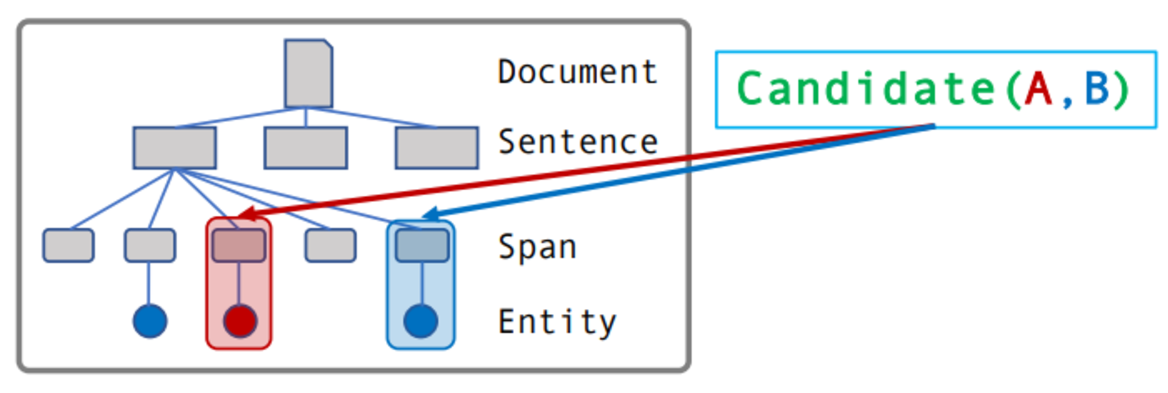
\includegraphics[width=\textwidth]{gfx/candidate.pdf}  }
	\caption{Modellazione del corpus in Snorkel.}
	\label{fig:methods:snorkel_struct}
\end{figure}

In Snorkel il corpus viene memorizzato come una gerarchia di oggetti della classe e tabella \textit{Context}. Attualmente la gerarchia predefinita per il testo è: \textit{Context -> Document -> Sentence -> Span} (Fig. \ref{fig:methods:snorkel_struct}).
Questa struttura viene definita e memorizzata nel database nelle successive operazioni della pipeline: nella fase di parsing si ottengono gli oggetti Document e Sentence e nella fase di candidate extraction si determinano le menzioni di entità Span che delimitano i segmenti di testo \textit{Candidate} per cui si vuole determinare un etichettamento.




\section{Parsing NLP}
\label{sec:methods:parsing_nlp}

Le triple Linked Data che si vogliono estrarre dal testo sono modellate secondo quella che in ambito linguistico viene chiamata \textit{proposizione}. Secondo la linguistica una proposizione può costituire una frase semplice se separata dal resto del discorso con simboli di \textit{interpunzione forte} o comporre insieme ad altre proposizioni una frase complessa. 

L'idea intuitiva è quella di analizzare tutte le frasi del corpus e distinguerne quelle che hanno features linguistiche tali da discriminare un particolare predicato e rappresentare un'asserzione Linked Data.

Per poter fare computazioni sul corpus risulta conveniente, come prima operazione, suddividere il corpus in frasi (semplici o complesse) che chiameremo d'ora in poi \textit{sentence}. Per ogni sentence si estraggono informazioni sintattiche, lessicali e semantiche che vengono poi sfruttate nei successivi passaggi della pipeline. 

\begin{figure}[htb]
	\fbox{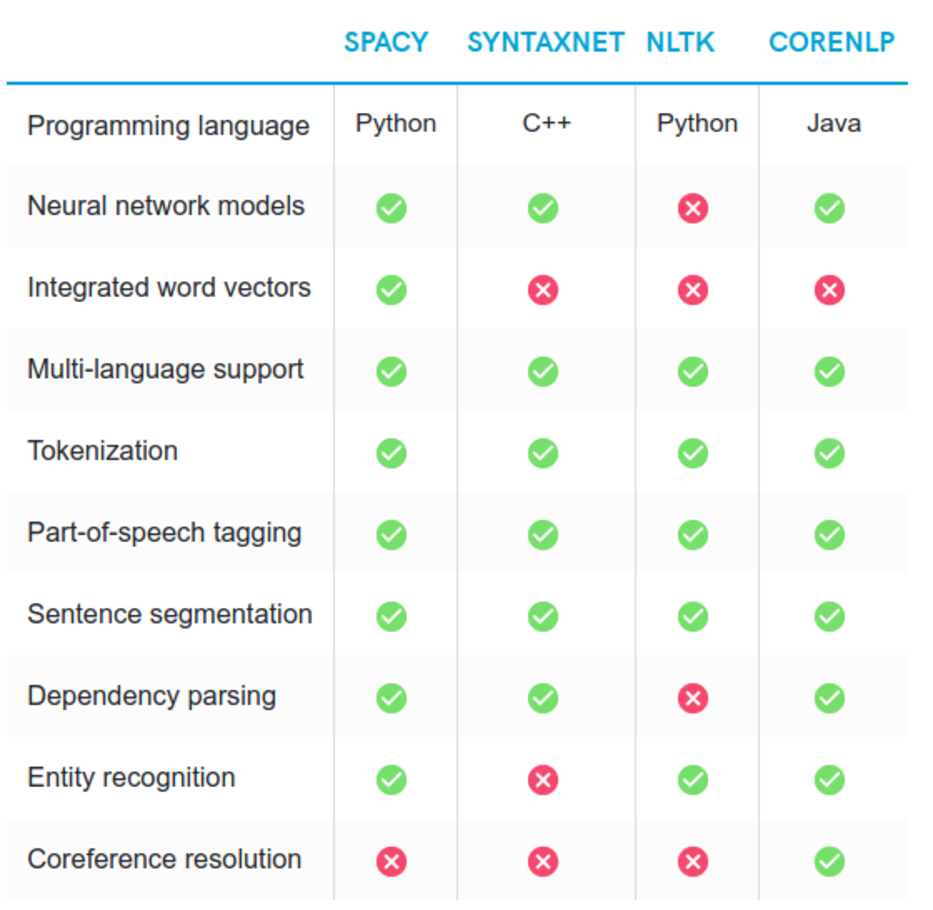
\includegraphics[width=\textwidth]{gfx/nlp_comparison.pdf} }
	\caption{Confronto delle funzionalità dei parser NLP più popolari.}
	\label{fig:methods:nlp_comparison}
\end{figure}

Il sistema Snorkel entra in azione sin da questo punto. Esso infatti integra due parser NLP: SpaCy e CoreNLP. Come dimostrato in \cite{Choi2015ItDD}, SpaCy è ad oggi il parser più veloce al mondo ed è quindi indicato il suo utilizzo con corpus molto grandi come in questo progetto. Non richiede comunque grandi compromessi in termini di precisione, rientrando infatti nell'1\% dei parser più precisi \cite{Spacyfacts}. Fornisce inoltre un output di feature linguistiche pensato per essere utilizzato come input per le più popolari librerie di deep learning utilizzate successivamente nella pipeline (Fig. \ref{fig:methods:nlp_comparison}).

Con le API di Snorkel è possibile processare corpus nei formati: XML, testo semplice, HTML e TSV. Integra inoltre il preprocessore testuale \textit{Apache Tika} per formati più complessi.

La fase di parsing produce come output una lista di riferimenti ai documenti processati memorizzata nella tabella \textit{Document} e una lista di frasi salvate nella tabella \textit{Sentence} con le relative feature linguistiche, che sono:
\begin{itemize}
\item indici dei caratteri iniziali e finali relativamente alla frase e al documento,
\item parole,
\item lemmi,
\item POS (Parts Of Speech),
\item dipendenze sintattiche,
\item NE (Named Entities),
\item tipi di NE.
\end{itemize}






















\section{Inferenza degli oggetti candidati}
\label{sec:methods:candidate_inference}
Un candidato (\textit{Candidate}) in Snorkel è un segmento di testo per il quale si vuole fare una previsione. I candidati vengono estratti prima della fase di labeling, scartando così le proposizioni grossolanamente inadatte a rappresentare la relazione da estrarre. Tale estrazione viene discriminata in funzione di feature linguistiche arbitrarie. Nel caso specifico, le frasi candidate sono solamente quelle che contengono tipi di named entity correlati al predicato considerato. Ad esempio, per la relazione \textit{dbo:spouse} le frasi candidate sono quelle che contengono almeno una coppia di named entity di tipo PERSON.

Avendo a che fare con triple, gli oggetti candidati da estrarre sono sempre delimitati da due named entity (\textit{Span}): il soggetto e l'oggetto. Si dice in questo caso che il candidato ha cardinalità 2.

I parser NLP condividono generalmente tra loro la stessa disponibilità e nomenclatura dei tipi di named entity più comuni, alcuni tipi più specifici invece potrebbero non essere sempre supportati. Il parser SpaCy fornisce i seguenti tipi:
\begin{itemize}
\item PERSON: persone vere o fittizie.
\item NORP: gruppi etnici, religiosi o politici.
\item FACILITY: edifici, aeroporti, strade, ponti etc.
\item ORG: organizzazioni, compagnie, agenzie, istituzioni etc.
\item GPE: paesi, città, stati.
\item LOC: località non GPE come località montuose o bacini acquiferi.	   \item PRODUCT: oggetti, veicoli, cibi etc.    
\item EVENT: battaglie, guerre, eventi sportivi o metereologici con un nome proprio.
\item WORK\_OF\_ART: titoli di libri, canzoni ed opere artistiche in generale.
\item LANGUAGE:	lingue.
\item DATE: date assolute o relative o periodi.
\item TIME: periodi di tempo minori di un giorno.	
\item PERCENT: valori percentuali.
\item MONEY: valori monetari.  
\item QUANTITY:	misurazioni come pesi o distanze.
\item ORDINAL: valori ordinali.
\item CARDINAL:	valori numerici diversi dagli altri tipi.
\end{itemize}

Questi tipi di named entity, pur non essendo usati in ambito Linked Data, hanno delle classi corrispondenti definite nelle ontologie OWL. In particolare, i tipi corrispondenti dell'ontologia di DBpedia vengono puntualmente utilizzati per la gran parte dei dati memorizzati nella base di conoscenza. E' stato costruito manualmente un mapping tra le classi OWL di DBpedia e i tipi di named entity corrispondenti.

A questo punto non resta che inferire quali classi OWL costituiscono il \textit{dominio} e il \textit{range} dei predicati in input. Dominio e range sono le classi attese (ma non obbligatorie) rispettivamente per il soggetto e l'oggetto del predicato.
Ad esempio, per il predicato \textit{dbo:birthPlace} che identifica il luogo di nascita di una persona, si ha dominio \textit{dbo:Person} e range \textit{dbo:Place}.

Il processo di inferenza di dominio e range viene attuato interrogando lo SPARQL Endpoint di DBpedia.
Alcuni predicati, come nel precedente esempio, hanno dominio e range unici definiti dalle proprietà \textit{rdfs:domain} e \textit{rdfs:range}, altri, più generici, possono averne molteplici e non specificati da tali proprietà. 
Nel primo caso il dominio e il range vengono ricavati direttamente. 
Nel secondo caso invece devono essere ricavati in maniera statistica. Per ogni predicato con dominio e range non unicamente definiti, si avvia un processo composto dalle seguenti operazioni:
\begin{enumerate}
\item ricavare i tipi di dato distinti che occorrono nelle triple,
\item contare tutte le triple,
\item contare le triple per ogni coppia di tipi di dominio e range,
\item considerare come valide le coppie di tipi con un occorrenza maggiore al 5\%, scartando così triple poco significative e probabilmente "rumorose".
\end{enumerate}

I tipi di dato Linked Data esaminati sono esclusivamente quelli mappati con i tipi di named entity. 

In questo modo sono stati ricavati indirettamente i tipi di named entity che sono relazionati con i predicati. Avendo questa informazione, si possono estrarre i candidati.

La ricerca di oggetti candidati viene svolta costruendo sotto-classi della classe \textit{Matcher} definita appositamente per ricercare il tipo di feature linguistica desiderata all'interno delle sentence. Sono stati costruiti matcher specifici per ogni tipo di named entity, parametrizzati per considerare esclusivamente gli \textit{n-grammi} di lunghezza massima pari a 7 e restituire solamente l'n-gramma più lungo per ogni matching consecutivo di named entity. Facendo un esempio, se vengono rilevate tre parole consecutive come "Rita Levi Montalcini" classificate come PERSON, viene restituito solamente l'intero n-gramma di lunghezza 3.

L'output della fase di candidate extraction è una lista di segmenti testuali delimitati dalle named entity, memorizzati nella tabella Span ed indicizzati in una tabella dinamicamente generata per ogni tipo di candidato.

Si noti che i candidati ottenuti e memorizzati possono essere riutilizzati per tutti quei predicati che hanno in comune lo stesso dominio e range. Ad esempio, i candidati delimitati dalle named entity di tipo PERSON e GPE sono adoperati sia per il predicato \textit{dbo:birthPlace} che per il predicato \textit{dbo:deathPlace}.















\section{Labeling Function}
\label{sec:methods:labelling}

Una volta filtrati, gli oggetti candidati diventano gli input che devono essere etichettati per formare l'insieme di training. Tale processo di labeling viene effettuato con quelle che in Snorkel vengono chiamate labeling function. 

Le labeling function sono essenzialmente funzioni Python passate come argomento all'oggetto della classe \textit{LabelAnnotator} che gestisce l'etichettamento. Questa classe indicizza sul database ogni labeling function ricevuta e procede successivamente ad eseguirle. Ogni segnale prodotto viene memorizzato nel database con il riferimento alla labeling function che l'ha generato.

I risultati di queste funzioni formano una matrice di etichette positive, negative o nulle. Successivamente, nella pipeline, tali etichette multiple verranno analizzate e gli verrà assegnata una probabilità marginale.

Esempi che possono essere pensati come fonti di weak supervision includono:
\begin{itemize}
\item euristiche specifiche del dominio;
\item distant supervision;
\item annotatori umani non esperti o non affidabili (\textit{Crowdsourcing}).
\end{itemize}
Queste tecniche sono utilizzabili in Snorkel sotto forma di labeling function. 

Nel caso di questo progetto la labeling functions su cui si fa maggiormente affidamento è la distant supervision e la si cerca di ottimizzare con varie labeling function basate su insiemi di parole chiave (\textit{bag of words}).

\subsection{Distant Supervision}
\label{sec:methods:labelling:distant_supervision}
Per poter effettuare la distant supervision bisogna essere in grado di interrogare la base di conoscenza su cui si fa affidamento. Nel caso specifico si fa nuovamente uso dello SPARQL Endpoint di DBpedia. Poichè lo SPARQL Endpoint è remoto ed interrogabile solamente via HTTP, la latenza nel tempo di interrogazione è alta. A tal proposito, tutte le triple di ogni relazione vengono estratte e memorizzate su database, una volta per tutte, prima di iniziare il processo di labeling.

Questa labeling function considera la coppia di named entity che delimita ogni candidato e restituisce un'etichetta positiva nel caso in cui viene trovata una corrispondente coppia di istanze nella base di conoscenza. 

Le menzioni testuali di un'entità nel testo non corrispondono esattamente al valore dell'entità salvata nella base di conoscenza. Ad esempio, all'entità menzionata come "Del Piero" corrisponde il valore memorizzato nella base di conoscenza come "Alessandro Del Piero". Snorkel non fornisce strumenti in grado di risolvere questo problema di entity linking che riduce drasticamente l'efficienza della distant supervision. A tale proposito, si è introdotto l'utilizzo del tool DBpedia Lookup e di confronti basati sulla similarità di stringhe. Utilizzando tale approccio si riesce quasi a triplicare la copertura della distant supervision proposta in Snorkel.

\subsubsection{DBpedia Lookup}
\label{sec:methods:labelling:distant_supervision:lookup}

Lookup è un progetto rilasciato da DBpedia che permette di effettuare ricerche basate su parole chiave sul database Linked Data. Tale ricerca permette anche di filtrare il tipo di entità desiderata. In tale modo effettuando una ricerca per la stringa "Del Piero" e filtrando per il tipo \textit{dbo:Person}, si ottengono i risultati con maggiore numero di riferimenti e di conseguenza, al primo posto, l'entità Linked Data con valore "Alessandro Del Piero". 

Al fine di effettuare un controllo ulteriore, si confronta la menzione testuale con il risultato restituito da Lookup tramite la misura di similarità tra stringhe \textit{Levenshtein} fornita dalla libreria \textit{Textacy}. Il valore soglia più appropriato per tale misura è stato valutato empiricamente.

\subsection{Euristiche specifiche}
\label{sec:methods:labelling:heuristic}  

La libreria Snorkel mette a disposizione delle funzioni "helper" che permettono la definizione di labeling function in grado di adattarsi alle particolarità delle relazioni da estrarre. In questo modo si può selezionare il contesto testuale da analizzare (il testo interno, alla destra o alla sinistra dello span candidato, le dipendenze sintattiche con altri candidati nella stessa frase etc.) e verificare delle condizioni arbitrarie con espressioni regolari, matcher o semplici confronti uno ad uno.

In un caso con dominio aperto come questo della LDKBP è importante definire delle labeling function basilari che possono essere riutilizzate per ogni predicato e valutare il loro impatto sul risultato finale. Per questo motivo si è preso in considerazione il progetto \textit{Spouse}\cite{snorkel_spouse_result_lfs} sviluppato dal team di Snorkel e introdotto nella sezione \ref{sec:literature_review:data_programming}.

Le labeling function sono state implementate in maniera analoga al progetto Spouse:
\begin{itemize}
\item \textit{LF\_distant\_supervision}: distant supervision che differisce da quella del progetto Spouse per l'uso di DBpedia Lookup per l'entity linking e la produzione di etichette negative in maniera pseudocasuale limitata al 15\% dei casi non positivi.
\item \textit{LF\_words\_between}: controllo della presenza di parole chiave positive che compaiono all'interno del candidato;
\item \textit{LF\_words\_right}: controllo della presenza di parole chiave positive che compaiono alla destra del candidato;
\item \textit{LF\_words\_left}: controllo della presenza di parole chiave positive che compaiono alla sinistra del candidato;
\item \textit{LF\_not\_words}: controllo della presenza di parole chiave negative che compaiono all'interno del candidato;
\item \textit{LF\_no\_word\_in\_sentence}: controllo dell'assenza di parole chiave positive all'interno dell'intera frase. 
\end{itemize}
Le ultime due funzioni restituiscono etichette negative o si astengono, le altre producono segnali positivi o si astengono.

Con la definizione di queste semplici labeling functions si prevede di aumentare la copertura della distant supervision e limitarne gli errori. In casi problematici più particolari è semplice definire funzioni di etichettamento ancora più specifiche.


\section{Training dei classificatori}
\label{sec:methods:training}

L'attività principale di Snorkel è la modellazione e l'integrazione
dei segnali ricchi di rumore forniti dalle labeling function.
Utilizzando l'approccio di data programming proposto, viene modellata la vera etichetta di classe per un dato come variabile latente in un modello probabilistico. Viene così stimata l'accuratezza di ogni tipo di labeling function.
Nel caso più semplice ogni funzione viene modellata come un "elettore" impreciso che è però indipendente dagli altri. In questo modo viene definito un \textit{modello generativo} degli output delle labeling function come segnali rumorosi sulla vera etichetta. Vengono anche modellate le dipendenze statistiche tra le funzioni per migliorare le prestazioni predittive. Per esempio, se due funzioni esprimono euristiche simili, questa dipendenza viene inclusa nel modello per evitare il problema del "doppio conteggio".

Il modello generativo implementato in Snorkel può essere allenato semplicemente fornendo come input la matrice dei segnali delle labeling function per ogni candidato. Nella fase di allenamento le funzioni vengono osservate e valutate in base a quanto concordano o discordano tra loro. Il modello allenato viene applicato sulla stessa matrice ottenendo un vettore delle probabilità marginali che viene salvato nel database.

Il vettore di probabilità marginali costituisce a sua volta l'input di allenamento del modello discriminativo. E' stata utilizzata una rete neurale di tipo \textit{Bi-LSTM} della libreria TensorFlow integrata in Snorkel. 

L'uso di questo particolare tipo di rete neurale è molto adatto ad ambiti come quello dell'analisi del testo. Per capirne il motivo si può fare un paragone con l'apprendimento umano: nella lettura di questa tesi, ad esempio, il lettore non reimposta la sua conoscenza ad ogni parola letta, ma interpreta ogni parola basandosi sulla comprensione dei concetti precedenti. Le reti neurali tradizionali non hanno memoria, mentre le \textit{Recurrent Neural Network (RNN)} e in particolare quelle composte da unità \textit{Long Short Term Memory} (\textit{LSTM}) affrontano questo problema delle \textit{dipendenze a lungo termine} rendendole particolarmente indicate a classificare informazioni con struttura sequenziale. Le RNN consentono il calcolo di rappresentazioni vettoriali a dimensione fissa per sequenze di parole di lunghezza arbitraria \cite{DBLP:journals/corr/PlankSG16}. Il vettore in output viene usato a sua volta come input per una RNN di livello superiore in una pila o gerarchia. Una RNN bidirezionale (\textit{Bi-RNN}) è un'estensione di una RNN che legge la sequenza di input due volte, dall'inizio alla fine e dalla fine all'inizio.
Le reti LSTM sono una variante delle reti RNN e sostituiscono le celle della RNN con celle LSTM che sono progettate appositamente per risolvere il problema noto come \textit{gradient vanishing}. Le reti \textit{Bi-LSTM} sono la controparte delle reti Bi-RNN basate su LSTM.

Sia nel classificatore generativo che in quello discriminativo gli iperparametri di allenamento non sono stati modificati rispetto a quelli di default consigliati nella documentazione di Snorkel.

E' possibile utilizzare degli insiemi di frasi etichettate manualmente per migliorare l'allenamento e quindi le prestazioni dei classificatori. Questa possibilità non è stata sfruttata perché sarebbe inattuabile a livello pratico generare tali insiemi in un caso reale di LDKBP considerato il vasto numero di predicati. Uno scopo di questo lavoro è proprio quello di valutare le prestazioni di Snorkel anche senza l'utilizzo di un insieme di tale genere. 

\section{Estrazione delle triple}
\label{sec:methods:triples_extraction}
La rete neurale allenata costituisce il mezzo per determinare la probabilità delle frasi non conosciute di rappresentare una delle relazioni Linked Data in input. 

Le frasi da classificare vengono inizialmente preprocessate, similmente alle frasi di training, estraendo features linguistiche e oggetti candidati.

Successivamente ogni candidato viene classificato con un grado di attendibilità per cui ci si aspetta che rappresenti la specifica relazione. I segmenti di testo con una probabilità maggiore ad un valore soglia diventano i candidati all'estrazione di nuove triple.

Dai candidati etichettati positivamente si estrae la tripla "grezza" composta dalla stringa soggetto, il predicato Linked Data e la stringa oggetto. Le stringhe soggetto e oggetto vengono ricercate con il servizio Lookup per effettuare l'entity linking. In caso di linking confermato dalla misura di similarità Levenshtein, si produce la tripla Linked Data.





%\begin{figure}[htb]
%	
\includegraphics[width=\textwidth]{gfx/Clean-Thesis-Figure}
%	\caption{Figure example: \textit{(a)} example part one, \textit{(c)} example part two; \textit{(c)} example part three}
%	\label{fig:system:example1}
%\end{figure}









\chapter{Test e Risultati}
\label{sec:results}


La pipeline sviluppata in questo lavoro è stata progettata per computare parallelamente input di grandi dimensioni e scalare in base alla potenza di calcolo e alla quantità di memoria a disposizione.
Per tale motivo si è rivelato conveniente effettuare test con un hardware molto performante messo a disposizione dal servizio di cloud computing \textit{Amazon EC2}. La macchina utilizzata è ottimizzata per il machine learning e consiste di 36 CPU virtuali e 60GB di memoria RAM.

Per facilitare il deploy del sistema sviluppato e dei servizi utilizzati ci si è serviti dell'infrastruttura di container Docker. In tale modo i test sono ripetibili in maniera omogenea e senza dipendere dalle caratteristiche dell'ambiente software utilizzato.

Brat è un sistema di annotazione manuale di \textit{gold labeling} che il team di Snorkel ha integrato nel progetto per annotare dati usati per valutare i test. Si tratta di un software in grado di gestire un archivio di documenti testuali e metterli a disposizione dell'utente che effettua l'annotazione tramite interfaccia web e tool grafici. L'integrazione fatta dal team di Snorkel consente di fare deploy su Brat dei documenti categorizzati come "test". In maniera altrettanto automatica, le annotazioni prodotte a mano in Brat vengono importate nel database di Snorkel. Tuttavia sono stati riscontrati dei problemi nel lancio del web server di Brat tramite le API di Snorkel. Per questo motivo si è utilizzato, anche in questo caso, l'immagine Docker ufficiale di Brat. Utilizzando lo stesso file system previsto dall'integrazione di Brat in Snorkel è stato possibile mantenere la validità dell'integrazione pur utilizzando il container Docker.

Il servizio Lookup ha dimostrato delle limitazioni in caso di esecuzione in ambiente hardware molto performante. Il servizio si è rivelato inadatto a ricevere parallelamente un elevato numero di richieste, aumentando gradualmente la latenza del tempo di risposta durante l'esecuzione della pipeline. A causa di tale problema si è fatto uso della componente Stack di Docker per replicare il servizio e distribuire il carico delle richieste in maniera bilanciata tra le varie repliche. Si è raggiunto un buon compromesso tra performance e consumo di memoria utilizzando 32 repliche del servizio e schedulando il riavvio periodico del servizio ogni 5 minuti.

I test sono stati condotti su un corpus ridotto di 100.000 frasi e i due predicati Linked Data \textit{dbo:birthPlace} e \textit{dbo:spouse}. 

La valutazione è stata svolta annotando 16 articoli di Wikipedia per le due relazioni. Gli articoli sono stati selezionati per essere rilevanti e insidiosi: si sono scelte solo pagine di persone e, in buona parte, sportivi per cui la presenza di named entity GPE è elevata e può mettere in difficoltà la distant supervision (es. la coppia "Totti"-"Roma" è un esempio negativo che la distant supervision è incapace di distinguere).

L'esecuzione dell'intera pipeline per ogni predicato ha impiegato un tempo medio di 19 minuti.



\section{Risultati}
\label{sec:results:results}

Una volta etichettati manualmente gli esempi di test con Brat, le utilità implementate in Snorkel permettono la valutazione automatica delle labeling function e del modello discriminativo finale.

Le labeling function vengono valutate in base alla copertura, alla coincidenza e ai conflitti dei segnali prodotti.
Facendo un confronto tra i risultati del progetto \textit{Spouse} condotto dal team di Snorkel \cite{snorkel_spouse_result_lfs} e quelli ottenuti per il predicato \textit{dbo:spouse} (Tab.\ref{tab:results:lfs1}) si può notare un aumento della copertura della distant supervision dall'1\% al 7\%. Questo risultato ha due motivazioni: l'impatto dell'entity linking eseguito con DBpedia Lookup, che incrementa la copertura al 3\% e la restituzione di un'etichetta negativa in maniera pseudocasuale. La validità di tale approccio è confermata dal valore dei conflitti che rimane stabilmente basso e quello delle sovrapposizioni che aumenta dal 0,9\% al 5,9\%.

I risultati riguardanti le labeling function per il caso \textit{dbo:birthPlace} (Tab. \ref{tab:results:lfs2}) mettono in luce come la sola distant supervision può essere inefficace in casi specifici come questo. In tal caso la copertura è bassa: risultato poco sorprendente vista la forte occorrenza di coppie persona-località negli esempi di test considerati. Ciò che maggiormente va considerato è il numero di conflitti della distant supervision dieci volte superiore al caso Spouse e pari al 50\% delle etichette positive restituite. Tali etichette, probabilmente inesatte, vengono bilanciate dalla presenza della labeling function che controlla la presenza di parole chiave negative.

\begin{table}[H]
\csvautobooktabular{csv/dbospouselfs.csv}
\caption{\textit{dbo:spouse}: statistiche delle labeling function.}
\label{tab:results:lfs1}
\end{table}

\begin{table}[H]
\csvautobooktabular{csv/dbobirthplacelfs.csv}
\caption{\textit{dbo:birthPlace}: statistiche delle labeling function.}
\label{tab:results:lfs2}
\end{table}




Le prestazioni del classificatore discriminativo sono riportate nella tabella \ref{tab:results:disc}. Analizzando le etichette prodotte si nota come per il predicato \textit{dbo:birthPlace} l'elevata presenza di falsi positivi è introdotta nelle stesse frasi che contengono un'etichetta vera positiva. In particolare, il caso più problematico è quello in cui oltre al luogo di nascita sono citati anche i nomi dei genitori. Questo schema ricorrente potrebbe essere rilevato da un'espressione regolare e quindi risolto da una labeling function specifica. In maniera simile, per il caso \textit{dbo:spouse} l'elevata presenza di falsi positivi è dovuta alla presenza di varie persone in frasi contenenti un'etichetta vera positiva, il caso più comune è quello della presenza dei nomi dei figli avuti dalla coppia. Anche in tal caso va valutato l'impatto di una labeling function apposita.
Un ulteriore tentativo di riduzione dei falsi positivi può essere fatto assegnando una distribuzione di probabilità a priori alle funzioni di labeling in fase di allenamento del modello generativo. Assegnando una probabilità a priori più elevata alla distant supervision si stima di ridurre i problemi appena menzionati.

\begin{table}[H]
\csvautobooktabular{csv/prf1_disc.csv}
\caption{ Statistiche modello discriminativo.}
\label{tab:results:disc}
\end{table}

La valutazione delle triple "grezze" estratte coincide con la valutazione del modello discriminativo. Il risultato allo stato dell'arte è rappresentato dal lavoro di \citet{Nguyen2011EndtoEndRE}. Per poter confrontare i due progetti in maniera significativa sarebbe opportuno svolgere training e test sugli stessi dati, tuttavia del progetto di \citet{Nguyen2011EndtoEndRE} si conoscono solamente gli otto predicati che hanno avuto risultati migliori. Di conseguenza sono stati usati per il confronto i risultati medi di precisione, richiamo e misura F1 che sono pari rispettivamente a 0.82, 0.56 e 0.67. I risultati medi del lavoro di questa tesi sono invece: precisione 0.52, richiamo 0.85, F1 0.63. Dal confronto si nota come l'approccio con sola distant supervision abbia un richiamo basso ma alta precisione, mentre la tecnica con labeling function sia meno precisa ma con un elevato richiamo. Questo fa sì che comunque la misura F1 sia quasi identica nei due progetti.

Le triple Linked Data estratte sono state valutate manualmente. Il numero totale di triple distinte estratte per il predicato \textit{dbo:birthPlace} è pari a 39 di cui 28 positive e 11 negative e per il predicato \textit{dbo:spouse} è pari a 22 di cui 15 positive e 7 negative.
Questo risultato mostra come il problema di entity linking influenza anche l'estrazione finale di triple dalle proposizioni etichettate positivamente. Si noti che non tutte le menzioni di entità estratte hanno una corrispondente entità in DBpedia e che alcune frasi etichettate positivamente sono ridondanti, questo implica che:
\begin{itemize}
\item le triple estratte sono di numero molto inferiore alla frasi etichettate positivamente;
\item molte frasi false positive non diventano triple poiché contengono menzioni a entità di secondaria rilevanza (nel caso specifico genitori o figli) che non sono presenti in DBpedia.
\end{itemize}
%\chapter{Sviluppi futuri}
\label{sec:discussion}

%\cleanchapterquote{Innovation distinguishes between a leader and a follower.}{Steve Jobs}{(CEO Apple Inc.)}



% !TEX root = ../my-thesis.tex
%
\chapter{Conclusioni e sviluppi futuri}
\label{sec:conclusion}

I test condotti sul progetto vanno ripetuti su un insieme più esteso di predicati e frasi, ma sembrano già confermare la possibilità di utilizzare un sistema simile in un ambiente di produzione di Linked Data.
 
I principali vantaggi del sistema proposto sono: 
\begin{itemize}
\item implementare facilmente un sistema di distant supervision;
\item migliorare le prestazioni della distant supervision;
\item ottenere risultati che approssimano lo stato dell'arte con un input testuale di piccole dimensioni;
\item possibilità di miglioramento iterativo dei risultati, applicando nuove parole chiave o labeling functions;
\item possibilità di modificare o sostituire modularmente i componenti della pipeline;
\item supporto multilingua;
\item scalabilità del sistema.
\end{itemize}

Un riscontro particolarmente interessante è quello di aver raggiunto risultati positivi pur mantenendo le configurazioni di default per i classificatori e senza utilizzare un insieme di supporto di esempi etichettati a mano. Questo consente l'utilizzo del progetto limitando l'apporto umano alla sola definizione di parole chiave e labeling function.
Questo risultato non toglie che debbano essere svolte ulteriori analisi sull'impostazione degli iperparametri di configurazione dei modelli di machine learning ed in particolare l'assegnazione della distribuzione di probabilità a priori delle labeling funcition nel modello generativo. 

I limiti maggiori sono stati individuati nell'entity linking e nella mancanza dell'utilizzo di tecniche di coreference resolution.

Il servizio DBpedia Lookup, pur essendo preciso, ha dimostrato di essere il collo di bottiglia della pipeline. Piuttosto che ripetere l'entity linking in ogni fase di labeling sarebbe forse più opportuno svolgerlo una volta per tutte in fase di estrazione dei candidati. Merita un ulteriore approfondimento la letteratura relativa (in particolare il survey di \citet{Shen2015EntityLW}) per trovare strumenti alternativi, altrettanto precisi, ma più rapidi.

Un aspetto decisivo è rappresentato dalla generazione di etichette negative. L'utilizzo di parole chiave negative migliora di molto le prestazioni, ma deve essere integrato con altri approcci. Nei prossimi sviluppi si cercherà di integrare la tecnica utilizzata da \citet{Mintz2009DistantSF} in cui vengono etichettati come negativi tutti quegli esempi che sono istanza di relazioni diverse da quella che si sta esaminando.

In futuro si cercherà inoltre di testare la pipeline su corpus in altre lingue. Questo può essere fatto semplicemente applicando diversi modelli linguistici per SpaCy e utilizzando corpus nella lingua scelta.

Vanno monitorati i progressi dei software di NLP nella tecnica di coreference resolution. In particolare SpaCy sembra essere attualmente al lavoro per integrare questa funzionalità \cite{spacy_coref} che potenzialmente avrebbe un impatto molto positivo su questo progetto.




%\input{content/chapter-introduction}   % INCLUDE: introduction
%\input{content/chapter-related-work}   % INCLUDE: related work
%\input{content/chapter-system}         % INCLUDE: system
%% !TEX root = ../my-thesis.tex
%
\chapter{Concepts: This text is here to test a very long title, to simulate the line break behavior, to show that an extremely long tilte also works}
\label{sec:concepts}

\cleanchapterquote{Users do not care about what is inside the box, as long as the box does what they need done.}{Jef Raskin}{about Human Computer Interfaces}

\Blindtext[2][1]

\section{Concepts Section 1}
\label{sec:concepts:sec1}

\Blindtext[2][2]

\section{Concepts Section 2}
\label{sec:concepts:sec2}

\Blindtext[3][2]

\section{Concepts Section 3}
\label{sec:concepts:sec3}

\Blindtext[4][2]

\section{Conclusion}
\label{sec:concepts:conclusion}

\Blindtext[2][1]
       % INCLUDE: concepts
%\input{content/chapter-conclusion}     % INCLUDE: conclusion

% --------------------------
% Back matter
% --------------------------
\appendix\cleardoublepage
%% !TEX root = ../my-thesis.tex
%
\chapter{Example Appendix}
\label{sec:appendix}

\Blindtext[1][1]

\section{Appendix Section 1}
\label{sec:appendix:sec1}

\Blindtext[1][1]

\begin{table}[h]
	\begin{tabularx}{\textwidth}{X | X | X}
		%\hline
		Alpha		& Beta			& Gamma			\\ \hline
		0			& 1				& 2				\\ \hline
		3			& 4				& 5				\\ %\hline
	\end{tabularx}
	\label{tab:table1}
	\caption{This is a caption text.}
\end{table}

\section{Appendix Section 2}
\label{sec:appendix:sec2}

\Blindtext[1][1]

\begin{table}[h]
	\begin{tabularx}{\textwidth}{X | X | X}
		%\hline
		Alpha		& Beta			& Gamma			\\ \hline
		0			& 1				& 2				\\ \hline
		3			& 4				& 5				\\ %\hline
	\end{tabularx}
	\label{tab:table2}
	\caption{This is a caption text.}
\end{table}

\Blindtext[1][2]
       % INCLUDE: appendix
%
{%
\setstretch{1.1}
\renewcommand{\bibfont}{\normalfont\small}
\setlength{\biblabelsep}{0pt}
\setlength{\bibitemsep}{0.5\baselineskip plus 0.5\baselineskip}
\printbibliography[nottype=online]
\printbibliography[heading=subbibliography,title={Webpages},type=online,prefixnumbers={@}]
}
\cleardoublepage

\listoffigures
\cleardoublepage

\listoftables
\cleardoublepage

\lstlistoflistings



% !TEX root = ../my-thesis.tex
%
%************************************************
% Declaration
%************************************************
\chapter*{Ringraziamenti}
\label{sec:declaration}
\thispagestyle{empty}


Ringrazio il mio babbo, la mia più grande fonte d'ispirazione per quello che sono oggi, la mia testa.\\
Ringrazio la mia mamma, il mio supporto più forte, il mio cuore.

Ringrazio le mie nonne, presenti in ogni istante con il loro affetto e le loro pietanze.

Ringrazio Benny per essere stata il mio unico appiglio per riuscire a mantenere la sanità mentale in questi mesi. Se scrivo questi ringraziamenti è grazie a te che mi rendi meno "orso".

Un grazie speciale va a Daniel e Ian, che sono... ve lo dico a voce che è meglio.

Grazie a Valerio, mio amico e guida nella mia (altrimenti disorganizzata) carriera universitaria.

Grazie alla professoressa Valentina Poggioni, per l'impeccabile disponibilità.





%*****************************************
%*****************************************

\clearpage
%\newpage
%\mbox{}

% **************************************************
% End of Document CONTENT
% **************************************************
\end{document}
